% Modelo UNISINOS para teses e dissertacoes

% PARA COMEÇAR A ESCREVER NÃO SE DETENHA AOS CÓDIGOS INICIAIS DO DOCUMENTO, VOCÊ IRÁ ENTENDÊ-LOS COM O TEMPO. 
% vÁ DIRETO PARA O CAPÍTULO 1 - INTRODUÇÃO.

% Arquivo de configurações e pacotes.
\input{0-setup}
% Nesse arquivo pode-se configurar a questão das páginas em branco para impressão em uma página (oneside) ou frente-verso (twoside). Quando utilizar a opção "oneside" não precisa utilizar a opção "openright".

% Arquivo de dados do documento: título, autor...
% ||||||||||||||||||||||||||||||||||||||||||||||
% Informações de dados para CAPA e FOLHA DE ROSTO
% ||||||||||||||||||||||||||||||||||||||||||||||
\titulo{Análise da Presença de Trihalometanos na Água para Consumo Humano do Estado do Rio Grande do Sul no período de 2014 a 2020} % Não utilize o ponto final no título
\autor{Rafaela Lorenzini}
\local{Porto Alegre}
\data{2021}
\orientador {Prof.ª Dr.ª Mariliz Gutterres Soares}
\coorientador{MSc. Luciano Barros Zini} % comente esta linha 


\instituicao{%
  UNIVERSIDADE FEDERAL DO RIO GRANDE DO SUL
  \par
  ESCOLA DE ENGENHARIA
  \par
  DEPARTAMENTO DE ENGENHARIA QUÍMICA
    \par
  TRABALHO DE DIPLOMAÇÃO EM ENGENHARIA QUÍMICA
}
\tipotrabalho{Monografia (Graduação)}
% O preambulo deve conter o tipo do trabalho, o objetivo, 
% o nome da instituição e a área de concentração 

\preambulo{Trabalho de Conclusão de Curso apresentado à COMGRAD/ENQ da Universidade Federal do Rio Grande do Sul como parte dos requisitos para a obtenção do título de Bacharel em Engenharia Química.}

%\preambulo{Trabalho apresentado como requisito para a obtenção do título de Mestre, pelo Programa de Pós-Graduação em Engenharia Elétrica da Universidade do Vale do Rio dos Sinos – UNISINOS.}

% ----------------------------------------------
% Configurações de aparência do PDF final
% ----------------------------------------------
% alterando o aspecto da cor azul


% ----------------------------------------------
% Início do documento
% ----------------------------------------------
\begin{document}

% ----------------------------------------------
% Adiciona lista de correções no início do documento.
% Comentar a linha abaixo quando o trabalho for concluído
% ----------------------------------------------

% ----------------------------------------------

% Arquivo de elementos pré-textuais: capa, folha de rosto, ficha catalografica, errata, folha de aprovação dedicatória, agradecimentos, epígrafe, resumos, lista de abreviaturas e siglas, lista de símbolos... 
% Seleciona o idioma do documento (conforme pacotes do babel)
%\selectlanguage{english}
\selectlanguage{brazil}

% Retira espaço extra obsoleto entre as frases.
\frenchspacing 

\newpage

% ==============================================
% ELEMENTOS PRÉ-TEXTUAIS
% ==============================================
\pretextual

% ----------------------------------------------
% Capa
% ----------------------------------------------
%\imprimircapa
% Capa personalizada sem o uso de \imprimircapa
\begin{capa} 
   \center
   \ABNTEXchapterfont\large\bfseries{\imprimirinstituicao} 
   \vfill
   %\vspace*{1cm}
   \ABNTEXchapterfont\large\bfseries\textsc{\MakeUppercase{\imprimirautor}}
   \vfill
   \begin{center}
   \ABNTEXchapterfont\Large\bfseries{\MakeUppercase{\imprimirtitulo}}
   \end{center}
   \vfill
   \vspace*{5cm}
   \large\bfseries\MakeTextUppercase{\imprimirlocal} \\
   \large\bfseries\imprimirdata
   \vspace*{1cm}
\end{capa}

% ----------------------------------------------
% Folha de rosto
% ----------------------------------------------
% folha de rosto personalizada sem uso de \imprimirfolhaderosto
%\makeatletter
%\renewcommand{\folhaderostocontent}{
%\begin{center}
 % {\ABNTEXchapterfont\large\imprimirautor}
  %\vspace*{\fill}%\vspace*{\fill}
  %\begin{center}
  %\ABNTEXchapterfont\bfseries\Large\imprimirtitulo
  %\end{center}
  %\vspace*{\fill}
  
  %\abntex@ifnotempty{\imprimirpreambulo}{%
   % \hspace{.45\textwidth}
    %\begin{minipage}{.5\textwidth}
    %\SingleSpacing
    %\imprimirpreambulo
    %\end{minipage}%
    %\vspace*{\fill}
  %}%

  %\abntex@ifnotempty{\imprimirorientador}{%
  %\hspace{.45\textwidth}
  %\begin{minipage}{.5\textwidth}
%	{\imprimirorientadorRotulo~\imprimirorientador}%
 % \end{minipage}%
  %}%
  
  %\begin{center}
  
   % \abntex@ifnotempty{\imprimircoorientador}{%
  %\hspace{.45\textwidth}
 % \begin{minipage}{.5\textwidth}
%	{\imprimircoorientadorRotulo~\imprimircoorientador}%
  %\end{minipage}%
  %}%
    


  
 % \vspace*{\fill}
  %{\abntex@ifnotempty{\imprimirinstituicao}{\imprimirinstituicao\vspace*{\fill}}}

  %{\large\imprimirlocal}
  %\par
  %{\large\imprimirdata}
 % \vspace*{1cm}
%\end{center}
%}
%\makeatother

% Folha de rosto (o * indica que haverá a ficha bibliográfica)
%\imprimirfolhaderosto*


\begin{folhadeaprovacao}

  \begin{center}
  {\ABNTEXchapterfont\large\imprimirautor}

  \vspace*{\fill}\vspace*{\fill}
   \begin{center}
    	\ABNTEXchapterfont\bfseries\Large\imprimirtitulo
    \end{center}
  \vspace*{\fill}

  \hspace{.45\textwidth}
    \begin{minipage}{.5\textwidth}
    	\imprimirpreambulo 
    \end{minipage}%




  %\vspace*{\fill}
   % \begin{flushleft}
  %	  Aprovado em 17 de Maio de 2021. \\
   % \end{flushleft}
 % \vspace*{\fill}
  
    %BANCA EXAMINADORA:% \imprimirlocal, \today :
  
   
   % Orientador\\
   %Coorientador \\
  % Prof. Dr. Jorge Otávio Trierweiler --  Avaliador UFRGS\\
  % MSc. Aristeu de Oliveira Junior --  Avaliador Externo
 %  MSc. Henrique Mezzomo --  Avaliador Externo
  
 
   %\assinatura{\textbf{Professor} \\ Convidado 4}
     
    \vspace*{\fill} \vspace*{\fill}
    \hspace{.5\textwidth}
    \begin{minipage}{.6\textwidth}
    	Orientadora:~\imprimirorientador \\
        Coorientador:~\imprimircoorientador
    \end{minipage}%
    
 
    \vspace*{\fill}
    \hspace{.4\textwidth}
    \begin{minipage}{1.5\textwidth}
    BANCA EXAMINADORA:\\
    	Prof. Dr. Jorge Otávio Trierweiler, Universidade Federal do Rio Grande do Sul \\
        MSc. Aristeu de Oliveira Junior, Ministério da Saúde\\
   MSc. Henrique Mezzomo, Secretaria Estadual de Saúde do Rio Grande do Sul
    \end{minipage}%
    \begin{center}
    \vspace*{0.5cm}
       {\large\imprimirlocal}
       \par
       {\large\imprimirdata}
       \vspace*{1.2cm}
       \end{center}
\end{center}
  
\end{folhadeaprovacao}

% ----------------------------------------------
% Inserir a ficha bibliografica catalográfica
% ----------------------------------------------
% Isto é um exemplo de Ficha Catalográfica, ou ``Dados internacionais de catalogação-na-publicação''. Você pode utilizar este modelo como referência. Porem, provavelmente a biblioteca da sua universidade lhe fornecerá um PDF com a ficha catalográfica definitiva após a defesa do trabalho. Quando estiver com o documento, salve-o como PDF no diretório do seu projeto e substitua todo o conteúdo de implementação deste arquivo pelo comando abaixo:

% \begin{fichacatalografica}
%     \includepdf{fig_ficha_catalografica.pdf}
% \end{fichacatalografica}
\begin{fichacatalografica}
	\sffamily
	\vspace*{\fill}					% Posição vertical
  	\begin{center}					% Minipage Centralizado
	\fbox{
    \begin{minipage}[t]{1,5cm} 
    \vspace{0.5cm} 
     %Algum número que o bibliotecario ira gerar
    \end{minipage}
    
    \begin{minipage}[t]{11cm}	% Largura
	\small
    \vspace{0.5cm}
	%\imprimirautor		% ATENCAO - SUBSTITUIR POR %Sobrenome, Nome do autor
    Lorenzini, Rafaela 
	
	\hspace{0.5cm} 
    \imprimirtitulo  / \imprimirautor. -- \imprimirdata.
	
	\hspace{0.5cm} 
    \pageref{LastPage} p. : il. (algumas color.) ; 30 cm.\\
	
    \hspace{0.5cm}
	\imprimirtipotrabalho~--~Universidade do Rio Grande do Sul, Departamento de Engenharia Química, Porto Alegre, RS, \imprimirdata. \hfill 
    
    \hspace{0.5cm}
    \imprimirorientadorRotulo~\imprimirorientador ;
    \imprimircoorientadorRotulo~\imprimircoorientador\\
	
	\hspace{0.5cm}
		1. Desinfecção
		2. Subprodutos de Desinfecção
		3. Trihalometanos
        \\
		%I. \imprimirtitulo \\
        %II. \imprimirorientador \\
    
%	\hspace{8.75cm} CDU 621.3 %algum outro numero
	
    \end{minipage}}
    
 %   \hspace{0.5cm}
  %  Dados Internacionais de Catalogação na Publicação (CIP) \\  	
   % (Bibliotecário: Nome Sobrenome – CRB 10/1298)
	
    \end{center}
\end{fichacatalografica}

% ----------------------------------------------
% Inserir errata
% ----------------------------------------------
% \begin{errata}
% Elemento opcional da \citeonline[4.2.1.2]{NBR14724:2011}. Exemplo:

% \vspace{\onelineskip}

% FERRIGNO, C. R. A. \textbf{Tratamento de neoplasias ósseas apendiculares com reimplantação de enxerto ósseo autólogo autoclavado associado ao plasma rico em plaquetas}: estudo crítico na cirurgia de preservação de membro em cães. 2011. 128 f. Tese (Livre-Docência) - Faculdade de Medicina Veterinária e Zootecnia, Universidade de São Paulo, São Paulo, 2011.

% \begin{table}[htb]
% \center
% \footnotesize
% \begin{tabular}{|p{1.4cm}|p{1cm}|p{3cm}|p{3cm}|}
%   \hline
%    \textbf{Folha} & \textbf{Linha}  & \textbf{Onde se lê}  & \textbf{Leia-se}  \\
%     \hline
%     1 & 10 & auto-conclavo & autoconclavo\\
%    \hline
% \end{tabular}
% \end{table}

% \end{errata}

% ----------------------------------------------
% Inserir folha de aprovação
% ----------------------------------------------
% Isto é um exemplo de Folha de aprovação, elemento obrigatório da NBR 14724/2011 (seção 4.2.1.3). Você pode utilizar este modelo até a aprovação do trabalho. Após isso, substitua todo o conteúdo deste arquivo por uma imagem da página assinada pela banca com o comando abaixo:
%
% \includepdf{folhadeaprovacao_final.pdf}
%


% ----------------------------------------------
% Dedicatória
% ----------------------------------------------
\newpage

\begin{dedicatoria}
\null
\vfill
\begin{flushright}
\hfill  {{\textit {Dedicado a minha família.}}}

\newpage
\end{flushright}
\end{dedicatoria}







% ----------------------------------------------
% Agradecimentos
% ----------------------------------------------
\begin{agradecimentos}

    Agradeço primeiramente à minha família, Antonino Lorenzini e Rosa Bernardete Lorenzini, por todo o amor e apoio dedicado a mim durante toda a minha vida e também ao meu irmão Charles Lorenzini por todo apoio, companheirismo e exemplo.
    
    À minha orientadora Prof.ª. Dr.ª Mariliz pelos ensinamentos e direcionamentos que balizaram este documento. Ao meu coorientador MSc. Luciano pelas
    reflexões e experiências que guiaram esta monografia. À Universidade Federal do Rio Grande do Sul pela qualidade e pelo ensino de excelência.
    
    Ao Centro Estadual de Vigilância em Saúde (CEVS), principalmente ao Programa da Vigilância da Qualidade da Água para Consumo Humano (VIGIAGUA) pelos dois anos de estágio de muito acolhimento e aprendizado em meio a uma pandemia. Agradecimento especial à Julce Clara da Silva, primeiro grande exemplo de engenheira química a seguir. Ao André Jarenkow, à Camila Bernardes Azambuja e ao Luciano Barros Zini, três grandes exemplos de engenheiros químicos. Todo meu carinho especial à Lisiane de Barros Trombin, mulher forte e com coração enorme. À Margot Vieceli e a Maria de Fátima Freitas Korndorfer pelo acolhimento desde o primeiro momento de estágio. Aos estagiários que comigo foram parceiros nessa jornada, Eduardo, Luana e Mariana. E a todos colegas do CEVS e VIGIAGUA. Além disso, quero agradecer e dizer que o VIGIAGUA pertence ao SUS.
    
    Finalmente, um grande agradecimento aos meus colegas de curso, aos meus amigos, e em especial à Ana Carolina por todo amor e companheirismo.
    
    
    
    
    
    
\end{agradecimentos}

% ----------------------------------------------
% Epígrafe
% ----------------------------------------------
% Importante: O autor da epígrafe deve constar na lista de referências
%\begin{epigrafe}
 %    \vspace*{\fill}
 %	\begin{flushright}
 %		\textit{``Os que se encantam com a prática sem a ciência \\
  %      são como os timoneiros que entram no navio sem timão nem bússola,\\
   %     nunca tendo certeza do seu destino."\\
%         (Leonardo da Vinci)}
 %	\end{flushright}
 %\end{epigrafe}

% ||||||||||||||||||||||||||||||||||||||||||||||
% RESUMOS
% ||||||||||||||||||||||||||||||||||||||||||||||

% ----------------------------------------------
% Resumo em português
% ----------------------------------------------
% Importante: De acordo com a NBR6024 as palavras-chaves devem ser separadas entre si por ponto e devem ter somente a primeira palavra escrita com letra maiúscula
\setlength{\absparsep}{18pt} % ajusta o espaçamento dos parágrafos do resumo
\begin{resumo}
	
Embora a desinfecção na água seja importante para remoção de patógenos, pode haver a geração de produtos secundários da desinfecção, onde destacam-se os trihalometanos (THMs). Estudos recentes sugerem a associação entre a exposição a longo prazo a THMs na água e câncer humano, como câncer de bexiga e colorretal. A taxa e o grau de formação de THMs aumentam em função da concentração de cloro e ácido húmico, temperatura, pH e concentração de íon brometo. O objetivo deste trabalho foi avaliar os resultados de presença de produtos secundários da desinfecção na água para consumo humano de sistemas de abastecimento de água do Rio Grande do Sul de 2014 a 2020, a partir dos dados de controle realizados pelos prestadores de serviço de abastecimento de água. Foram avaliados 17.245 análises, onde 8.761 tiveram presença de THMs. A água dos sistemas abastecidos por manancial superficial apresentaram maior concentração de THMs comparada ao manancial subterrâneo e misto. 33 municípios apresentaram presença de THMs com concentração acima do valor máximo permitido (0,1 $mg.L^-^1$), o que corresponde a 1.925.192 pessoas expostas pelo menos em algum momento entre 2014 a 2020. A correlação de Spearman mostrou que o aumento de chuva ou temperatura ocasiona um aumento de concentração de THMs. Ao avaliar os compostos de THMs entre 2014 e 2015, as concentrações foram maiores para clorofórmio e bromodiclorometano. Como possíveis ações para reduzir a concentração de THMs pode-se otimizar a clarificação para remoção de precursores, reduzir a concentração de cloro ou substituir o produto de desinfecção.

 
   
	\vspace{\onelineskip}
 
	\noindent 
	\textbf{Palavras-chaves}: Desinfecção. Produtos secundários da desinfecção (PSD). Trihalometanos (THM). 
\end{resumo}

% ----------------------------------------------
% Resumo em inglês
% ----------------------------------------------
% Importante: De acordo com a NBR6024 as palavras-chaves devem ser separadas entre si por ponto e devem ter somente a primeira palavra escrita com letra maiúscula
\begin{resumo}[Abstract]
\begin{otherlanguage*}{english}
	Although disinfection in water is important for the removal of pathogens, there may be the generation of secondary disinfection products, in which trihalomethanes (THM) stand out. Recent studies suggest an association between long-term exposure to trihalomethanes in water and human cancer, such as bladder and colorectal cancer. The rate and degree of THMs formation increase depending on chlorine and humic acid concentration, temperature, pH, and bromide ion concentration. The objective of this work was to evaluate the results of the presence of secondary products of disinfection in water for human consumption of water supply systems in the Rio Grande do Sul from 2014 to 2020, based on the control data carried out by water supply service providers. 17,245 analyzes were evaluated, where 8,761 had the presence of THMs. The water in the systems supplied by surface water showed a higher concentration of THMs compared to the underground and mixed water sources. 33 municipalities showed the presence of THMs with a concentration above the maximum allowed value (0.1 $mg.L^-^1$), which corresponds to 1,925,192 people exposed at least some time between 2014 and 2020. Spearman's correlation showed that the increase in rain or temperature causes an increase in THMs concentration. When evaluating THMs compounds between 2014 and 2015, the concentrations were higher for chloroform and bromodichloromethane. As possible actions to reduce the THMs concentration, the clarification can be optimized to remove precursors, reduce the chlorine concentration or replace the disinfection product. 
    
	\vspace{\onelineskip}
 
	\noindent 
	\textbf{Key-words}: Disinfection. Disinfection byproduct (DBP). Trihalomethanes (THMs). 
\end{otherlanguage*}
\end{resumo}

% ----------------------------------------------
% resumo em francês 
% ----------------------------------------------
% Importante: De acordo com a NBR6024 as palavras-chaves devem ser separadas entre si por ponto e devem ter somente a primeira palavra escrita com letra maiúscula
% \begin{resumo}[Résumé]
%  \begin{otherlanguage*}{french}
%     Il s'agit d'un résumé en français.
 
%    \textbf{Mots-clés}: latex. abntex. publication de textes.
%  \end{otherlanguage*}
% \end{resumo}

% ----------------------------------------------
% resumo em espanhol
% ----------------------------------------------
% Importante: De acordo com a NBR6024 as palavras-chaves devem ser separadas entre si por ponto e devem ter somente a primeira palavra escrita com letra maiúscula
% \begin{resumo}[Resumen]
%  \begin{otherlanguage*}{spanish}
%    Este es el resumen en español.
  
%    \textbf{Palabras clave}: latex. abntex. publicación de textos.
%  \end{otherlanguage*}
 
% \end{resumo}

% ----------------------------------------------
% inserir lista de ilustrações (ou figuras)
% ----------------------------------------------
\pdfbookmark[0]{\listfigurename}{lof}
\listoffigures*
\cleardoublepage

% Diferentes tipos de listas podem ser criadas por meio de macros do memoir.

% ----------------------------------------------
% inserir lista de tabelas
% ----------------------------------------------
\pdfbookmark[0]{\listtablename}{lot}
\listoftables*
\cleardoublepage

% ----------------------------------------------
% inserir lista de quadros (ex.: \begin{quadro} \end{quadro})
% ----------------------------------------------
% \pdfbookmark[0]{\listofquadrosname}{loq}
% \listofquadros*
% \cleardoublepage

% ----------------------------------------------
% inserir lista de abreviaturas e siglas
% ----------------------------------------------
% Importante: As abreviaturas e siglas devem estar em ordem alfabética
\begin{siglas}
\item[CONAMA] Conselho Nacional do Meio Ambiente
\item[CORSAN] Companhia Riograndense de Saneamento
\item[COD] Carbono Orgânico Dissolvido
\item[COT] Carbono Orgânico Total
\item[ETA] Estação de Tratamento de Água
\item[EUA] Estados Unidos da América
\item[HA] Haloaldeído 
\item[HAA] Ácido Haloacético
\item[HAN] Haloacetonitrilo
\item[HAconAm] Haloacetamida
\item[HK] Halocetona
\item[HNM] Halonitrometano
\item[IARC] Agência Internacional de Pesquisa em Câncer
\item[INMET] Instituto Nacional de Meteorologia
\item[LD] Limite de Detecção
\item[LQ] Limite de Quantificação
\item[MOA] Matéria Orgânica Aquagênica
\item[MON] Matéria Orgânica Natural
\item[MOP] Matéria Orgânica Pedogênica
\item[MS] Ministério da Saúde
\item[pH] Potencial Hidrogeniônico
\item[PDF] Formato de Documento Portátil
\item[POA] Processo Oxidativo Avançado
\item[PSD] Produtos Secundários da Desinfecção
\item[SAA] Sistema de Abastecimento de Água
\item[SH] Substâncias Húmicas
\item[SISAGUA] Sistema de Informação de Vigilância da Qualidade da Água para Consumo Humano
\item[THM] Trihalometanos
\item[USEPA] Agência de Proteção Abiental dos Estados Unidos 
\item[UV] Ultravioleta 
\item[VMP] Valor Máximo Permitido
\item[WHO] World Health Organization

\end{siglas}


% ----------------------------------------------
% inserir lista de símbolos
% ----------------------------------------------
% Importante: Os símbolos devem estar na ordem de aparecimento no texto.
%\begin{simbolos}
 % \item[$ \Gamma $] Letra grega Gama
  %\item[$ \Lambda $] Lambda
 % \item[$ \zeta $] Letra grega minúscula zeta
 % \item[$ \in $] Pertence
%\end{simbolos}

% ----------------------------------------------
% inserir o sumário
% ----------------------------------------------
\pdfbookmark[0]{\contentsname}{toc}
\tableofcontents*
\cleardoublepage


% ----------------------------------------------
% ELEMENTOS TEXTUAIS
% ----------------------------------------------
\textual

% ----------------------------------------------
% Exemplo de capítulo sem numeração, mas presente no Sumário
% ----------------------------------------------
%\chapter*[Introdução]{Introdução}
%\addcontentsline{toc}{chapter}{Introdução}
% ----------------------------------------------

% ||||||||||||||||||||||||||||||||||||||||||||||
% CAPITULO 1 - INTRODUÇÃO
% ||||||||||||||||||||||||||||||||||||||||||||||
% Nas seções e subseções a primeira letra de cada palavra devem estar em maiúsculas.
%\chapter{Introdução}\label{Introdução}



%\todo[inline]{Alguns manuais de pacotes latex foram adicionados na pasta manuals}

%\todo[inline, color=red]{Procure se informar a respeito do Mendeley. É um software para gerenciar referencias bibliográficas que irá facilitar muito a inclusão das referências no documento. Procure também como importar as referencias inseridas no mendeley para o arquivo references.bib aqui no overleaf}

%Este documento e seu código-fonte são exemplos de referência de uso da classe \textsf{abntex2} e do pacote \textsf{abntex2cite}. O documento exemplifica a elaboração de trabalho acadêmico (tese, dissertação e outros do gênero) produzido conforme a ABNT NBR 14724:2011 \emph{Informação e documentação - Trabalhos acadêmicos - Apresentação}.

%A expressão ``Modelo Canônico'' é utilizada para indicar que \abnTeX\ não é modelo específico de nenhuma universidade ou instituição, mas que implementa tão somente os requisitos das normas da ABNT. Uma lista completa das normas observadas pelo \abnTeX\ é apresentada em \citeonline{abntex2classe}.


%Este documento deve ser utilizado como complemento dos manuais do \abnTeX\ \cite{abntex2classe,abntex2cite,abntex2cite-alf} e da classe \textsf{memoir} \cite{memoir}. 

%Esperamos, sinceramente, que o \abnTeX\ aprimore a qualidade do trabalho que você produzirá, de modo que o principal esforço seja concentrado no principal: na contribuição científica.


%\begin{align}
%  B'&=-\nabla \times E,\\
%  E'&=\nabla \times B - 4\pi j,
%\end{align}

%\begin{equation} 
% f(x) n=(x+a)(x+b)
%\end{equation}

%\section{Justificativa}

%\begin{figure}[htp]
%	\centering
%	\caption{\label{fig:met-disc-fig01} No centro da figura é representado um logo $U_1$.} 
%	\includegraphics[width = 0.8\linewidth]{images/unisinos.png}
%	\legend{Fonte: Desenvolvido pelo autor.}
%\end{figure}

%\section{Delimitação do trabalho}

%\section{Objetivos}

%Matematicamente, o Fator de Potência (FP) pode ser expresso como:
%\begin{equation}
%	\label{eq:k-55}
 %   {
  %  \displaystyle 
   % FP = \frac{\cos(\varphi)}{\sqrt{1 - THD^2}}
    %}
%\end{equation}

%\subsection{Objetivos gerais}

%\subsection{Objetivos específicos}

%%%%%%%%%%%%%%%%%%%%%%%%%%%%%%%%%%%%%%%%%%%%%%%%%
% Capitulo de exemplos utilizando arquivo externo 
%%%%%%%%%%%%%%%%%%%%%%%%%%%%%%%%%%%%%%%%%%%%%%%%%
%\include{abntex-exemplos} % comente esta linha para facilitar, mas não apague o arquivo abntex-exemplos.tex pois ele contém exemplos interessantes que podem auxiliar na elaboração da dissertação.

% ||||||||||||||||||||||||||||||||||||||||||||||
% CAPITULO 1
% ||||||||||||||||||||||||||||||||||||||||||||||
\chapter{Introdução} \label{Introdução}



A água é um recurso essencial no apoio e manutenção da saúde humana e no desenvolvimento das atividades sociais e econômicas. O crescimento populacional, a urbanização, a industrialização, a agricultura e as mudanças no padrão de consumo têm gerado demandas cada vez maiores por recursos de água doce em todo o mundo \cite{UNESCO2021}. A ingestão de água potável de má qualidade pode levar a vários riscos à saúde, sendo um dos principais vetores de organismos causadores de doenças, por isso, a desinfecção deve ser considerada indispensável e prioritária sempre que a água estiver
contaminada \cite{brasila}.

A desinfecção é uma etapa crucial no tratamento da água para consumo humano com intuito de promover a eliminação ou inativação de organismos possivelmente patogênicos, que após o processo de clarificação ainda estejam presentes \cite{who17}. Entretanto, é necessário encontrar um equilíbrio entre a eficiência da desinfecção e a formação de produtos secundários da desinfecção indesejáveis na água destinada ao consumo humano para que ela atenda ao padrão de potabilidade brasileiro. A reação de formação ocorre entre a matéria orgânica natural oxidada (substâncias húmicas) e produtos químicos utilizados na desinfecção \cite{DU201751}. Além disso, as principais causas da formação de produtos secundários da desinfecção é causada pela diminuição da qualidade dos recursos hídricos, o aumento da demanda de água e lançamento de efluentes no meio ambiente pelas atividades industriais, agrícolas e centros urbanos sem acesso a saneamento \cite{sun2016characteristics}. 


Os trihalometanos (THMs) mais comumente presentes em água potável são triclorometano (clorofórmio), tribromometano (bromofórmio), bromodiclorometano e dibromoclorometano, que em 1974, foram  identificados como os primeiros produtos secundários da desinfecção em água desinfetada  \cite{bellar1974occurrence} e, no mesmo ano, o clorofórmio foi relatado  \cite{rook1974}. Desde então, há mais de 700 produtos secundários da desinfecção relatados na literatura. No entanto, a maior presença nos produtos secundários da desinfecção se deve aos trihalometanos e ácidos haloacéticos. Além disso, em 1976, o Instituto Nacional do Câncer dos Estados Unidos da América publicou resultados mostrando que o clorofórmio era cancerígeno em animais de laboratório \cite{national1976report}. Estudos recentes sugerem a associação entre a exposição a longo prazo a trihalometanos na água e câncer humano, como câncer de bexiga e colorretal \cite{cancer,cancerdebexiga}.

A legislação brasileira de potabilidade da água, por meio do Anexo XX da Portaria de Consolidação N° 5 do Ministério da Saúde de 28 de setembro de 2017, pouco comenta e recomenda sobre os produtos secundários da desinfecção, limitando-se a fixar 0,1 $mg.L^-^1$ para trihalometanos totais como um valor máximo permitido para águas tratadas e distribuídas em sistemas de abastecimento de água \cite{AnexoXX}, sem diferenciação entre os quatro componentes formadores dos trihametanos (bromodiclorometano, bromofórmio, clorofórmio e dibromoclorometano), somente a soma total.

O presente estudo avaliou a presença de produtos secundários da desinfecção em água para consumo humano no Estado Rio Grande do Sul entre 2014 e 2020, ao que se refere a trihalometanos e  em relação a aspectos como população abastecida, manancial de captação (superficial, subterrâneo e misto), estágio da água em função do ponto de coleta (água bruta, tratada e distribuída), sazonalidade e condição climática. 


\chapter{Objetivos} \label{Objetivos}
\section{Objetivo Geral}
O presente trabalho tem o objetivo geral de avaliar os resultados retirados dos dados de controle da qualidade da água realizados pelos responsáveis pelo abastecimento público quanto a presença de THMs na água para consumo humano de sistemas de abastecimento de água do Rio Grande do Sul.

\section{Objetivos Específicos}

\begin{itemize}
  \item	Determinar o cumprimento do plano de amostragem de THMs e atendimento ao padrão brasileiro de potabilidade para estes subprodutos de desinfecção da  série histórica de 2014 a 2020 do Estado do Rio Grande do Sul;

  
  \item Determinar a proporção de ocorrência de THMs entre tipos de manancial e pontos de coleta;
  \item	Determinar os municípios e a população que foi exposta a água não potável em função de concentrações de THMs superiores ao valor máximo permitido;
  \item Determinar aspectos relacionados à sazonalidade e se há correlação de presença de THMs com a condição climática;
  \item Para 2014 e 2015 avaliar separadamente, a partir de relatórios da CORSAN, o que há de presença para cada um dos quatro componentes do THM.

\end{itemize}
 





% ||||||||||||||||||||||||||||||||||||||||||||||
% CAPITULO 2
% ||||||||||||||||||||||||||||||||||||||||||||||
\chapter{Revisão Bibliográfica} \label{Revisão Bibliográfica}
Neste capítulo serão tratados tópicos necessários para o entendimento do que será exposto no trabalho. Nesta seção está reunido o que se encontra na literatura da área a respeito de sistema de abastecimento e tratamento da água, precursores e formação de produtos secundários da desinfecção com ênfase nos trihalometanos.

\section{Sistema de Abastecimento de Água}
Os sistemas de abastecimento de água (SAA) para consumo humano são assim definidos por possuírem instalação composta por um conjunto de obras civis, materiais e equipamentos, desde a zona de captação até as ligações prediais, destinada à produção e ao fornecimento coletivo de água potável, por meio de rede de distribuição \cite{AnexoXX}. Além das obras de engenharia, os SAA devem também operar com eficiência a fim de proteger a população abastecida contra os riscos à saúde humana. Em um SAA, o controle de riscos à saúde inicia-se na escolha do manancial de onde é captada a água, sendo que devem ser priorizados mananciais com menos impacto ambiental, protegidos de contaminação de natureza química ou biológica por processos antrópicos \cite{brasila}.

Os SAAs são responsáveis pela maior parte do abastecimento de água no Rio Grande do Sul. Em 2021, a população abastecida por SAA corresponde a 9.714.040 de habitantes (85,38\%) dos 11.377.239 de habitantes do estado \cite{sisagua}. Além disso, possui 32 sistemas integrados de abastecimento de água, com sistemas que abastecem mais de um município, ou seja, o município onde está localizado o SAA abastece municípios adjacentes a ele. Também pode ocorrer de um único município haver mais de um SAA e água ser misturada nas redes de abastecimento de distribuição \cite{Brasil1}.

\section{Captação de Água}
As captações variam de acordo com condições locais, hidrológicas, topográficas e hidrogeológicas \cite{brasilb}. Nos tópicos a seguir são descritas as formas de captação superficial e subterrânea. 

\subsection{Captação de Águas Superficiais}

Mananciais superficiais são cursos d'água, represas e lagos  \cite{brasila} e devem preencher os requisitos mínimos de aspectos quantitativos e qualitativos do ponto de vista físico, químico e biológico \cite{Tsutiya}. As precipitações atmosféricas são responsáveis por abastecer as depressões naturais do terreno (lagos) ou represamentos artificiais, ou escoam superficialmente e alimentam os cursos d’água (córregos, ribeirões, rios). Outra parcela infiltra-se no solo, constituindo os mananciais subterrâneos, os quais alimentam os mananciais superficiais \cite{brasilb}.  

A Resolução CONAMA Nº 357 de 2005 classifica os corpos hídricos e determina aqueles suscetíveis à captação de água para consumo humano: águas doces de classe especial, classe 1, classe 2 e classe 3. Da classe especial para a classe 3, a concentração dos parâmetros da qualidade da água vai diminuindo e consequentemente o tratamento necessário vai se tornando mais complexo devido à concentração de substâncias indesejadas \cite{conama357}. Quanto maior é o grau de proteção do manancial a ser captada a água para consumo humano e da bacia hidrográfica em conjunto com suas nascentes, menos etapas de tratamento são necessárias, dada a melhor qualidade da água bruta. No entanto, esses mananciais vêm sofrendo degradações, principalmente devido ao avanço da urbanização e a carência de coleta e tratamento de esgoto. Geralmente as áreas mais protegidas encontram-se distantes de centros urbanos, o que aumenta o custo de bombeamento.     

A captação de água em manancial superficial é a etapa inicial e engloba a estrutura construída junto ao corpo hídrico para a retirada de água. Essas obras devem ser projetadas e construídas a fim de funcionar ininterruptamente, com qualidade e quantidade suficiente para o abastecimento e devem possuir acesso facilitado para a operação e manutenção do sistema \cite{Tsutiya}. A captação pode ser direta ou indireta. Os principais fatores para a definição do manancial superficial e do tipo de captação são a qualidade da água bruta, vazão mínima necessária e os custos das estruturas de captação, adução e tratamento. A captação indireta se dará pela construção de reservatórios de acumulação de água, sendo representadas por barragens e represas para que os períodos chuvosos cubram o déficit de água das épocas de estiagem \cite{brasilb}.

\subsection{Captação de Águas Subterrâneas}

Fontes de água encontrada abaixo da superfície do solo são classificadas em lençóis ou aquíferos, não confinados (freáticos) e confinados (artesianos). A captação ocorre em poços rasos ou profundos, galerias de infiltração ou nascentes, dentre outras formas \cite{brasilb}. O lençol não confinado (freático) está localizado entre a superfície do solo e uma camada impermeável (rocha), submetido à pressão atmosférica, normalmente de menor profundidade e consequentemente de menor custo de escavação. O lençol confinado (artesiano) encontra-se confinado entre camadas impermeáveis,  geralmente possui maior profundidade em relação ao lençol freático, e submetido a pressão superior à atmosférica  \cite{brasila}.

A água bruta obtida por captação subterrânea, por consequência da percolação através dos interstícios granulares do solo, permite na maioria dos casos, dispensar em quase totalidade as operações unitárias de tratamento necessárias na captação superficial, restringindo-se à desinfecção, fluoretação e eventual correção de pH. Outro ponto favorável à captação subterrânea é que na maioria dos casos dispensa bombeamento de água bruta, pois a desinfecção pode ser instalada próxima ao poço \cite{brasila}.

A Resolução CONAMA Nº 396 de 2008  classifica águas subterrâneas e determina aqueles que devem ser utilizados para a captação de água para consumo humano: as águas subterrâneas de classe especial, classe 1, classe 2, classe 3 e classe 4. Da classe especial a classe 4, a concentração dos parâmetros da qualidade da água vão diminuindo, consequentemente o tratamento necessário vai se tornando mais complexo \cite{conama396}. A alteração da qualidade do manancial deve-se a atividades antrópicas. O lençol freático (poços rasos) possui a possibilidade de contaminação por fontes pontuais como fossas, postos de gasolina e outras fontes de poluição difusas. Na maioria dos casos, a contaminação de águas subterrâneas ocorre em função da inexistência de redes coletoras de esgoto \cite{brasila}.


\section{Tratamento da Água}
O tratamento da água para consumo humano tem a finalidade de adequar as características da água aos padrões de potabilidade exigidos pelo Ministério da Saúde (MS) por meio do Anexo XX da Portaria de Consolidação Nº 5 de 2017. O tratamento possui objetivos como a prevenção de doenças de veiculação hídrica, de origem microbiológica ou química, e prevenir a cárie dentária por meio da fluoretação. A sequência de etapas mais utilizadas em uma estação de tratamento de água (ETA) de ciclo completo ou convencional pode incluir: coagulação, floculação, sedimentação (ou flotação), filtração, desinfecção, fluoretação e correção de pH \cite{brasilb}. 

\begin{figure}[h]
\caption{\small Representação esquemática de um sistema de abastecimento de água (SAA) convencional.}
\includegraphics[scale=0.55]{images/tratamento da agua.png}
\legend{\footnotesize Fonte: Adaptado \cite{usepa99}.}
\label{fig01}
\end{figure}


A clarificação consiste em processos unitários de coagulação, floculação, decantação (sedimentação) e filtração. Essa etapa remove partículas, incluindo microrganismos (bactérias, vírus e protozoários). É importante que os processos sejam otimizados e controlados para permitir um desempenho consistente e confiável \cite{who17}. Esse conjunto de operações destinado à remoção de partículas em suspensão via sedimentação. promove a manutenção das condições físico-químicas da água.

A coagulação é uma etapa indispensável para a remoção satisfatória de partículas e outros contaminantes que são responsáveis pela turbidez, cor, odor e sabor nas águas para consumo humano. Também apresenta um grande significado na remoção de matéria orgânica, o que resulta em menor produção de subprodutos de desinfecção, como os trihalometanos e ácidos haloacéticos. Os principais agentes coagulantes utilizados são sulfato de alumínio, policloreto de alumínio, cloreto férrico, sulfato ferroso e hidróxido de cálcio.

Na etapa da floculação, ocorre a aglutinação de partículas pequenas em flocos maiores, ganhando tamanho e densidade, não ocorre remoção de impurezas, o que é feito nos decantadores ou filtros. Na decantação, os flocos com impurezas e partículas ficam depositados no fundo dos decantadores, de onde o lodo acumulado deve ser removido periodicamente em operações de limpeza dos decantadores \cite{brasilb}. 

Águas provenientes de manancial superficial devem ser submetidas a processo de filtração \cite{AnexoXX},pois essa operação pode funcionar como uma barreira eficiente para a remoção de microrganismos patogênicos, em alguns casos ser a única barreira de tratamento \cite{who17}. A filtração é a passagem de água por um leito filtrante de material granular, por meio do qual ocorre a remoção de partículas não retiradas no decantador. A seleção do filtro será em função da qualidade da água bruta e cada alternativa corresponderá a uma granulometria adequada para o leito filtrante, os filtros são classificados de acordo com o fluxo, ascendente e descendente, e em função da velocidade de filtração, rápida ou lenta \cite{brasilb}. O valor máximo permitido de turbidez após a filtração é de: 0,5 uT para a filtração rápida (tratamento completo ou filtração direta) e 1,0 uT para a filtração lenta \cite{AnexoXX}. Também há os tratamentos avançados, entre eles a filtração por membrana (microfiltração, ultrafiltração, nanofiltração e osmose reversa), no entanto, são processos com custos elevados e com isso, ainda pouco utilizados no Brasil.

A desinfecção é o processo de destruição ou inativação de microrganismos pela aplicação de um agente de desinfecção de caráter físico ou químico. Dentre os quais os mais empregados são: oxidantes químicos, como o cloro, dióxido de cloro e ozônio, e radiação ultravioleta  \cite{brasilb}. Na sequência será dado um detalhamento maior para o processo de desinfecção.

A fluoretação da água dos sistemas de abastecimento para consumo humano consiste em adicionar concentrações do íon fluoreto na água, a fim de produzir efeitos desejados à prevenção de cárie dental \cite{AnexoXX}. A aplicação é realizada por meio de aparelhos dosadores, sendo inseridos o fluoreto de sódio, o fluossilicato de sódio ou o ácido fluossilícico \cite{brasilb}.  De acordo com o Anexo XXI da Portaria de Consolidação N°5 do MS/2017, o valor máximo permitido para a concentração de íon fluoreto é de 1,5 $mg.L^-^1$ \cite{AnexoXX} e pela Portaria Nº 10 da Secretaria da Saúde do Rio Grande do Sul de 1999, este valor deve permanecer entre 0,6 a 0,9 $mg.L^-^1$ \cite{ses99}.

A maioria das ETAs possui correção de pH, já que o próprio tratamento da água tende a abaixar o mesmo. A correção ocorre pela adição de cal hidratada ou carbonato de sódio que servirá para corrigir a alcalinidade da água, e preservar a rede de distribuição de corrosão. A água tratada deve manter seu pH estabilizado entre 6 a 9,5 nas redes de distribuição \cite{brasilb}.


\section{Desinfecção da Água}

Nos anos de 1880, em Londres, o Dr. John Snow conduziu o caso mais famoso de estudo epidemiológica, comprovando empiricamente a relação água consumida com a transmissão da cólera. Após mais de 100 anos, hoje há uma lista extensa de potenciais doenças de veiculação hídrica devido à presença de microrganismos patogênicos, incluindo bactérias, protozoários, vírus, microalgas e cianobactérias. O primeiro uso do cloro em processo contínuo é datado antes de 1900 em estações de tratamento de água na Bélgica e na Inglaterra. Após a introdução de filtros e desinfecção em ETAs dos EUA, as doenças de veiculação hídrica foram praticamente erradicadas, como é o caso da febre tifóide e da cólera. Em Nova York, entre os anos de 1911 e 1915, o número de mortes por febre tifóide eram de 185 a cada 100 mil habitantes e este número foi para zero com a introdução dos processos de filtração e desinfecção com cloro \cite{brasila,usepa99}.

Com intuito de promover a desinfecção da água para consumo humano é necessário que se utilizem mecanismos para a eliminação ou inativação de possíveis patógenos, que após os processos antecedentes do tratamento ainda estejam presentes na mesma por meio de um agente químico ou físico. Esses microrganismos são responsáveis por doenças de veiculação hídrica, por isso, a desinfecção deve ser considerada indispensável e prioritária sempre que a água estiver contaminada \cite{brasila}. Além disso, a eficiência da desinfecção é resultante da oxidação ou ruptura da parede celular dos microrganismos, decorrente da desintegração das células e da difusão de um agente no interior da mesma, o qual interfere na sua atividade. A desinfecção é um processo seletivo que não destrói todas as formas vivas e nem elimina todos os organismos patogênicos, a destruição completa das formas vivas é denominada esterilização \cite{dibernardo2017}.

Os desinfetantes possuem um papel fundamental numa estação de tratamento de água e devem apresentar as seguintes características que promovem a desinfecção: destruir, em tempo hábil, os organismos patogênicos na quantidade e nas condições em que se apresentam; não ser tóxico, não causar odor e sabor; ter custo razoável e oferecer condições seguras de transporte, armazenamento, manuseio e aplicação; ter concentração na água medida de forma rápida, através de métodos simples e confiáveis; produzir residuais persistentes, assegurando a qualidade da água contra eventuais contaminações na rede de abastecimento  \cite{dibernardo2017}.

Dentre os principais desinfetantes, utilizados na estações de tratamento de água para consumo humano no Rio Grande do Sul, destaca-se o cloro, pois é um dos métodos mais comuns para desinfecção de água devido ao seu potencial de oxidação eficaz, custo-benefício e simplicidade de operação. São usados para fins de cloração o cloro gasoso, hipoclorito de sódio e hipoclorito de cálcio \cite{Meyer}. A hidrólise desses desinfetantes produz ácido hipocloroso \begin{math}(HOCl)\end{math} e íon hipoclorito \begin{math} (OCl^- )\end{math} que são definidos como cloro livre.  Além desses, a monocloroamina \begin{math}(NH_2Cl)\end{math} e a dicloramina  \begin{math}(NHCl_2)\end{math} também são encontradas, o que é chamado de cloro combinado. \cite{brasila}. De acordo com a Organização Mundial da Saúde (OMS), recomenda-se dosagens de \begin{math}0,2 - 0,5 mg.L^-\end{math} de cloro no processo de desinfecção, essas doses são consideradas adequadas para manter um cloro residual livre de \begin{math}0,2 mg.L^-\end{math} após o tratamento e na rede de distribuição \cite{who17}. 

Nas últimas décadas tem-se procurado alternativas ao cloro, decorrente da possibilidade de formação de produtos secundários da desinfecção, tais como compostos halogenados que podem causar riscos à saúde pública, verificados quando o cloro livre está presente e a água contém precursores, normalmente matéria orgânica natural, geralmente substâncias húmicas. Entre essas alternativas será abordado brevemente os desinfetantes ozônio e dióxido de cloro. 

A Agência de Proteção Ambiental dos Estados Unidos (USEPA) descreve, por meio do \textit{Safe Water Treatment Rule}, critérios exigidos na desinfecção em sistemas de abastecimento público superior a 10 mil habitantes, tais como 3 log de inativação de cistos de \textit{Giardia}, 4 log de inativação de vírus e 2 log de inativação de \textit{Cryptosporidium}. Além disso, sugere os valores máximos permitidos dos residuais cloro e dióxido de cloro, respectivamente, 4 mg $Cl_2$/L e 0,8 mg $ClO_2$/L. Na Tabela 1, é apresentado um resumo dos principais desinfetantes e seu desempenho.

\begin{table}[!htb]
\begin{center}
\small
\caption{Principais desinfetantes/oxidantes e suas condições}
    \begin{tabular}{l|c|c|c}
    \toprule
        \textbf{Condição}  & \textbf {Cloro} & \textbf{Ozônio} & \textbf{Dióxido de cloro}\\\hline
      Produz THM em água COT   & S & AV & N \\
      Produz compostos orgânicos oxidados & AV & S & AV \\
      Produz subprodutos inorgânicos & N & AV & S \\ 
      Produz compostos orgânicos bromados & AV & S & AV \\ 
      Interferência da turbidez & AV & S & AV \\ 
      Inativação de \textit{Giardia} > 2 log & N & S & S \\ 
      Inativação de \textit{Cryptosporidium} > 2 log & N & S & N \\ 
      Inativação de vírus > 2 log & S & S & S \\ 
      Habilidade do operador (1:baixa; 5:alta) & 1 & 5 & 5 \\ 
      Aplicável para instalações médias ou grandes & S & S & S \\ 
      \bottomrule
    \end{tabular}
    \legend{\footnotesize S: Sim; N: Não; AV: às vezes. Fonte: Adaptado de \cite{usepa99}.}
    \label{tab01}
\end{center}
\end{table}
Como mostra na Tabela 1, a escolha de um desinfetante ou a combinação de alguns deles depende essencialmente da qualidade da água bruta, a concentração de carbono orgânico dissolvido (COD) e de brometos, principalmente quando a pré-desinfecção for necessária. Na desinfecção final, o agente deve garantir a produção de água isenta de organismos patogênicos, como \textit{Escherichia Coli}, cistos de  \textit{Giardia}, oocistos de \textit{Cryptosporidium}, e vírus \cite{usepa99}; \cite{dibernardo2017}. Além disso, analisando a Tabela 1 observa-se que o ozônio é o desinfetante mais eficiente para a maior parte dos microrganismos patogênicos encontrados em águas superficiais destinadas ao abastecimento. Entretanto, devido ao custo de implantação, operação e manutenção relativamente alta, o dióxido de cloro pode ser uma alternativa , nas quais há necessidade de pré-desinfecção e a água bruta possui precursores da formação de compostos orgânicos halogenados. As principais vantagens e desvantagens dos desinfetantes usados no tratamento de água encontram-se resumidos na Tabela 2.

\begin{table}[!htb]
\begin{center}
\small
\caption{Vantagens e desvantagens dos desinfetantes usados no tratamento da água para consumo humano.} \label{tab:com_esp}
\begin{tabular}{p{2cm}p{6.25cm}p{6.25cm}}
\toprule
\textbf{Desinfetante} & \textbf{Vantagens} & \textbf{Desvantagens} \\
\midrule
Cloro & Oxidante poderoso; sistema de dosagem relativamente simples; residual persistente; uso comum & Forma compostos orgânicos halogenados quando a água possui precursores; problemas de sabor e odor; influência do pH na formação de espécies de cloro\\ \hline
\addlinespace[2pt]
Ozônio & Oxidante poderoso; geralmente forma quantidades pequena de compostos orgânicos halogenados; não apresenta problemas de odor e sabor; pequena influência do pH; ajudante de coagulação & Meia-vida curta; geração no local da ETA; consumo excessivo de energia elétrica; produz alguns compostos biodegradáveis; complexa geração e medição de residuais nos meios gasoso e líquido; corrosivo\\ \hline
\addlinespace[2pt]
Dióxido de cloro & Oxidante poderoso; residual relativamente persistente; geralmente forma quantidades pequenas de compostos orgânicos halogenados; não há influência do pH & Formação de alguns compostos organohalogenados (diferentes dos trihalometanos); possíveis subprodutos (clorito e clorato); geração no local da ETA\\
\bottomrule
\end{tabular}
\legend{\footnotesize Fonte: Adaptado de \cite{usepa99}.}
\end{center}
\end{table}

\section{Precursores de Produtos Secundários da Desinfecção}

Os precursores de produtos secundários da desinfecção são definidos como uma mistura de compostos orgânicos e inorgânicos que podem formar produtos secundários da desinfecção em algum ponto no processo de desinfecção, vindos de fontes naturais ou antropogênicas \cite{chen2010predicting}. Exceto para a matéria orgânica natural que deve estar na reação de formação, vários produtos químicos e contaminantes na água, como agrotóxicos, produtos farmacêuticos, agentes antibacterianos, estrogênios, corantes têxteis, surfactantes, antibióticos e produtos de cuidados pessoais, algas, produtos microbianos solúveis, aminoácidos, também servem como precursores significativos de produtos secundários da desinfecção \cite{lan2018genotoxicity}.

Precursores inorgânicos, como  \begin{math} B^-\end{math}, \begin{math}  I^- \end{math}, e outros íons inorgânicos não receberam preocupação suficiente em comparação com precursores produtos secundários da desinfecção orgânicos. Brometo e iodeto são componentes mais reativos a formação de subprodutos da desinfecção, que por sua vez podem ser ainda mais tóxicos do que seus equivalentes clorados \cite{Krasner2006,zhao2016effects}. 

A matéria orgânica natural (MON) representa toda matéria orgânica existente nos mananciais diferindo da matéria orgânica e dos compostos de origem antrópica. Cerca de 20\% da MON consiste em compostos orgânicos com estrutura química definida, como carboidratos, aminoácidos e hidrocarbonetos. Os restante (80\%) correspondem a massa de matéria orgânica detríticas, pertencentes a um grupo de estrutura química indefinida, com tempo de residência mais longo no ambiente e relativamente resistente à degradação; são denominadas matéria orgânica refratária (MOR). A matéria orgânica natural pode ser classificada de acordo com a origem das plantas, que serviram como material de partida para a formação desses compostos. A matéria orgânica natural aquagênica (MOA) é aquela formada na água, pela excreção e decomposição de plâncton e bactérias aquáticas, ao passo que a pedogênica (MOP) refere-se à decomposição de plantas terrestres e de microrganismos, incluindo material lixiviado dos solos e aportado nos sistemas aquáticos.
A MOP é formada pela degradação de lignina, carboidratos e proteínas, os quais levam à formação de compostos aromáticos (especialmente substâncias carboxílicas, fenólicas e benzênicas) e, em menor quantidade, de compostos alifáticos. A matéria orgânica encontrada em lagos e rios é predominantemente decorrente de processo de lixiviação da MOP do solo. Desta forma, processos unicamente de MOA ocorrem apenas em águas oceânicas \cite{rocha2009}. Substâncias húmicas (SH) são os principais constituintes da matéria orgânica natural (MON), globalmente distribuídas em ambientes terrestres e aquáticos. Estima-se que cerca de 50\% do carbono orgânico dissolvido (COD) em águas superficiais e oceânicas consiste em matéri orgânica refratária do tipo SH \cite{swietlik2004reactivity, rocha2009}.

A presença de MON cria sérios problemas à qualidade da água e seus processos de tratamento. Esses problemas incluem efeito negativo na qualidade da água devido à cor, sabor e odor; aumento dos requisitos de dosagem de coagulante e desinfetante, o que por consequência aumenta o lodo e produz subprodutos de desinfecção; promove crescimento biológico no sistema de distribuição e aumento de metais pesados complexados e poluentes orgânicos adsorvidos \cite{mon1995}. Algumas medidas da existência de MON podem ser efetuadas por parâmetros indiretos que fornecem informações importantes, como a análise de carbono orgânico total (COT) ou carbono orgânico dissolvido (COD); a absorbância da radiação UV específica, que é a absorbância medida no comprimento de onda de 254nm dividida pela concentração de COD; potencial de formação de THM; THMs de amostras coletadas em diferentes pontos do sistema de abastecimento de água; e oxigênio consumido \cite{dibernardo2017}. A maior parte da MON pode ser removida pela coagulação e floculação seguida de sedimentação e filtração, outras opções de tratamento para a remoção adsorção com carvão ativado, técnicas de filtração por membrana e processos de oxidação avançados \cite{mon1995}.






\section{Produtos Secundários da Desinfecção}

O uso de cloro como desinfetante no tratamento de água potável para inativar o patógeno reduziu muito as doenças transmitidas pela água, como cólera e febre tifóide. No entanto, as reações entre desinfetantes e matéria orgânica na água bruta podem produzir produtos secundários da desinfecção (PSDs), também relatados como subprodutos da desinfecção \cite{Abbas2014}, muitos deles são relatados como carcinogênicos, mutagênicos, citotóxicos e genotóxicos \cite{benson2017disinfection}. Os primeiros PSDs identificados em água desinfetada foram os trihalometanos (THMs) \cite{bellar1974occurrence} e o clorofórmio foi relatado em água potável clorada em 1974 \cite{rook1974}. Desde então, mais de 700 PSDs foram relatados na água desinfetada. Os PSDs são classificados entre alifáticos e aromáticos, os alifáticos incluem: trihalometanos (THMs), ácidos haloacéticos (HAAs), halocetonas (HKs), haloaldeídos (HAs) e PSDs nitrogenados, como haloacetonitrilos (HANs), halonitrometanos (HNMs) e haloacetamidas (HAconAms); e PSDs aromáticos incluem: fenólicos e heterocíclicos. Como mostra a Tabela 3, a desinfecção com cloro produz PSDs halogenados, não halogenados e inorgânicos, enquanto o dióxido de cloro produz somente PSDs inorgânicos.

\begin{table}[!htb]
\begin{flushleft}
\small
\caption{Desinfetante e sua formação de produtos secundários da desinfecção na água para consumo humano.} \label{tab:com_esp}
\begin{tabular}{p{3cm}p{5cm}p{2.5cm}p{4cm}}
\toprule
\textbf{Desinfetante} & \textbf{Produtos Organohalogênicos} & \textbf{Produtos Inorgânicos} & \textbf{Produtos não halogenados} \\
\midrule
Cloro, hipoclorito de sódio, hipoclorito de cálcio & THMs, HAAs, HANs, HKs, HAs, N-cloraminas, clorofenóis, cloropicrina, hidratos de cloral, furanonas de halo, bromoidrinas & Clorato & Aldeídos, ácidos carboxílicos, benzeno, ácido alcanóico, ácido ciano alcanóico\\ \hline

Dióxido de cloro &  & Clorito, Clorato & Desconhecido\\ 
\bottomrule
\end{tabular}
\legend{\footnotesize Fonte: Adaptado de \cite{who17}}
\end{flushleft}
\end{table}

A equação geral para a formação de THMs e outros PSDs halogenados, se há presença de MON e brometos é descrita a seguir: 
\begin{equation}
\mathrm{HClO}+\mathrm{Br}^{-}+\mathrm{MON}
  \rightarrow
  \mathrm{THMs} + \mathrm{PSDs} 
\end{equation}
A MON é o principal precursor com quem os halogênios reagem para formar subprodutos. Na ausência íons brometos, somente PSDs clorados são formados, na presença destes, o ácido hipocloroso os oxida rapidamente a ácido hipobromoso $HBrO$, o qual, juntamente com o residual de ácido hipocloroso, formam os compostos que possuem cloro e bromo \cite{dibernardo2017}. A formação de PSDs dependente do inúmero de fatores influentes como: dosagem de cloro aplicada; temperatura; pH; tempo de contato; conteúdo de matéria orgânica; turbidez; nutrientes (nitrogênio, fósforo e enxofre); residual de cloro livre e concentrações de brometos; e tipo de o material do tubo \cite{Abbas2014,LI2019335}.

\begin{table}[!htb]
\begin{flushleft}
\small
\caption{Dados regulamentados com base na toxicidade e valor máximo permitido.} \label{tab:com_esp}
\begin{tabular}{p{0.9cm}p{3.8cm}p{2.5cm}p{1cm}p{1.5cm}p{1.75cm}p{1.5cm}}
\toprule
\textbf{PSDs} & & \textbf{Grupo de Câncer$^b$ (EPA)} & \textbf{OMS} & \textbf{USEPA} ($mg.L^-^1$) & \textbf{União Europeia} ($mg.L^-^1$) & \textbf{Brasil} ($mg.L^-^1$) \\
\midrule
THM4 & & & & 0,08 & 0,1 & 0,1\\ 
& Clorofórmio & B2 & 0,3 & 0,07 & & \\ 
& Bromodiclorometano & B2 & 0,06 & 0 & & \\ 
& Clorodibromometano & C & 0,1 & 0,06 & & \\
& Bromofórmio & B2 & 0,1 & 0 & & \\
\hline
HAA5 & & & & 0,06 & & 0,08\\
& Ácido dicloroacético & B2 & 0,05 & 0 & &\\
& Ácido trihloroacético & C & 0,2 & 0,02 & & \\
& Ácido monocloroacético & D & 0,02 & 0,07 & &\\
& Ácido monobromoacético & D & $^a$ & & & \\
& Ácido dibromoacético & D & $^a$ & & & \\\hline
HANS & & & & & & \\
& Dibromoacetonitrila & C & 0,07 & & & \\
& Dicloroacetonitrila & C & 0,02 & & & \\
& Bromocloroacetonitrila & & $^a$ & & &\\
& Tricloroacetonitrila & & $^a$ & & &\\\hline
HKs & & & & & & \\
& Cloroacetonas (1,1-dicloroacetona) & & $^a$ & & &\\\hline
HAs  & & & & & & \\
& Tricloroacetaldeído & C & 0,01 & & & \\\hline
PSD fenil & & & & & & \\
& 2- clorofenol & D & $^a$ & & &\\
& 2,4-diclorofenol & D & $^a$ & & &\\
& 2,4,6-triclorofenol & B2 & 0,2 & & & 0,02\\
\bottomrule
\end{tabular}
\legend{\footnotesize $^a$ Dados inadequados disponíveis para definir os valores de referência.\\ 
$^b$ B2 = Provável carcinógeno humano com base em dados suficientes de estudos com animais; C = Possível carcinógeno humano; D = Não classificado como cancerígeno para humanos de acordo com \cite{iarc2004}.\\

Fonte: Adaptado de \cite{Kali2021}.}
\end{flushleft}
\end{table}

\newpage
No Brasil, diante da necessidade de controle dos PSD, o Anexo XX da Portaria de Consolidação nº 5 do Ministério da Saúde de 2017 — define como valor máximo permitido (VMP) a concentração de 0,1 mg.L\- para THM, 0,08  mg.L\- para HAA e 0,02 para 2,4,6-triclorofenol, conforme mostra a Tabela 4, juntamente com os dados de toxicidade dos PSDs. O número mínimo de amostras e frequência de coleta para o controle da qualidade da água de SAA, a respeito dos THMs, depende do tipo de manancial, para o manancial superficial: saída do tratamento - 1 análise trimestral, sistema de distribuição - o número de análises depende da população abastecida, quando for menor que 50 mil habitantes, 1 análise trimestral, e quando for maior que 50 mil habitantes, 4 análises trimestrais; para o manancial subterrâneo: é dispensada a análise na saída do tratamento, sistema de distribuição o número de análises depende da população abastecida, quando for menor que 50 mil habitantes, 1 análise anual, e quando for maior que 50 mil habitantes, 1 análise semestral. A análise de PSDs é dispensada no ponto de captação. A Portaria GM/MS Nº 888, de 4 de maio de 2021 que alterou o Anexo XX da Portaria de Consolidação nº 5 do Ministério da Saúde de 2017, modificou a frequência de análises e adicionou outro PSD formado a partir da cloração, o 2,4-diclorofenol. A Tabela 5 resume como é a legislação e como ficará a partir da publicação referente ao número mínimo de amostras e frequência .


\begin{table}[!htb]

\small
\centering
\caption{Número mínimo de amostras e frequência para os PSDs pelo Anexo XX da Portaria de Consolidação Nº 5/2017 e a Portaria Nº 888/2021.} 
\begin{tabular}{cccccccccl}
\toprule
\multirow{2}{*}{Portaria} & \multirow{2}{*}{Manancial} & \multicolumn{2}{c}{Saída do Tratamento} & \multicolumn{6}{c}{Sistema de Distribuição} \\
 &  & Nº Amostras & Frequência & \multicolumn{3}{c}{Nº Amostras} & \multicolumn{3}{c}{Frequência} \\\midrule
PRC 5/2017 & Superficial & 1 & Trimestral & 1$^a$ & 4$^b$ & 4$^c$ & \multicolumn{3}{c}{Trimestral$^a^b^c$} \\
PRC 5/2017 & Subterrâneo & \multicolumn{2}{c}{Dispensada a análise} & 1$^a$ & 1$^b$ & 1$^c$ & Anual$^a$ & \multicolumn{2}{c}{Semestral$^a^b$} \\\hline
Port. N° 888/2021 & Superficial & \multicolumn{2}{c}{Dispensada a análise} & 1$^a$ & 4$^b$ & 8$^c$ & \multicolumn{3}{c}{Bimestral$^a^b^c$} \\
Port. N° 888/2021 & Subterrâneo & \multicolumn{2}{c}{Dispensada a análise} & 1$^a$ & 2$^b$ & 3$^c$ & Anual$^a$ & \multicolumn{2}{c}{Semestral$^a^b$}\\\bottomrule
\end{tabular}
\legend{\footnotesize $^a$ <50.000 habitantes abastecidos; $^b$ 50.000 a 250.000 habitantes abastecidos; $^c$ >250.000 habitantes abastecidos. }

\end{table}


Para a redução de PSDs, vários pontos devem ser considerados durante a seleção de estratégias de controle, ou seja, eficiência no processo, eficácia de custo e riscos potenciais à saúde. A coagulação e a otimização do processo de desinfecção são técnicas econômicas. No entanto, adsorção com carvão ativado, tecnologias de membrana, processos oxidativos avançados (POAs) e tratamentos combinados são métodos caros, mas eficientes para o controle de PSDs \cite{Kali2021}.




\section{Trihalometanos (THMs)}

Os trihalometanos (THMs) são compostos de carbono único substituídos por halogênio com fórmula geral $CHX_3$, onde X representa um halogênio, que pode ser flúor, cloro, bromo ou iodo, ou combinações dos mesmos. Os THMs mais comuns presentes na água potável são triclorometano (clorofórmio), tribromometano (bromofórmio), bromodiclorometano e dibromoclorometano \cite{who2005}, no padrão de potabilidade brasileiro é considerado como trihalometanos total \cite{AnexoXX}. 

São formados na água potável principalmente como resultado da cloração de produtos de matérias orgânicas presentes em fontes de água bruta. A taxa e o grau de formação de THM aumentam em função de concentração de cloro e ácido húmico, temperatura, pH e concentração de íon brometo \cite{stevens1976}. Bem como sendo o THM mais comum, o clorofórmio também é o principal produto secundário da desinfecção em água potável clorada. Na presença de brometos, THMs bromados são formados preferencialmente e as concentrações de clorofórmio diminuem \cite{saidan2016effect}.

A exposição ocorre por ingestão de água potável, inalação pelo ar pela volatilização da água, vias de absorção dérmica e ingestão por alimentos. Eles possuem diferentes propriedades físico-químicas e toxicológicas \cite{villanueva}. Os quatro compostos de THMs são líquidos à temperatura ambiente. Eles variam entre relativamente e extremamente volátil, com pressões de vapor a 25°C variando de 0,8 kPa para o bromofórmio a 23,33 kPa para o clorofórmio \cite{who2005}. 

O clorofórmio é usado como solvente e na produção de outros produtos químicos \cite{who2004}. O bromodiclorometano é usado na síntese de outros produtos químicos e como solvente, enquanto o dibromoclorometano é um intermediário na fabricação de refrigerantes, agrotóxicos, propelentes e outros produtos químicos orgânicos. O bromofórmio é usado na síntese de farmacêuticos, como solvente, e nas indústrias de aeronaves e construção naval como um ingrediente em produtos químicos resistentes ao fogo e fluido de medição. Os THMs são lançados no ambiente como fontes industriais \cite{who2005}.

Em 1974, Rook e outros relataram a identificação dos primeiros PSDs em água potável clorada: clorofórmio e outros trihalometanos (THMs) \cite{rook1974}. Em 1976, a Agência de Proteção Ambiental dos EUA (USEPA) publicou os resultados de uma pesquisa nacional que mostrou que o clorofórmio e os outros THMs eram onipresentes na água potável clorada. No mesmo ano, o National Cancer Institute publicou resultados mostrando que o clorofórmio era cancerígeno em animais de laboratório \cite{national1976report}. Além disso, os primeiros relatórios apareceram no final dos anos 1970, mostrando que os extratos orgânicos de água potável eram mutagênicos no ensaio de mutagenicidade de \textit{Salmonella} \cite{loper1980mutagenic}.  Eles não são mutagênicos, mas têm efeitos cancerígenos e outros efeitos tóxicos graves em humanos \cite{Abbas2014}. Há estudos que sugerem que há uma associação significativa entre a exposição a longo prazo a THMs na água e câncer humano, como câncer de bexiga, colorretal \cite{cancerdebexiga}. Além disso, estudos recentes indicaram que os THMs podem causar outros efeitos à saúde, por exemplo, retardo do crescimento intrauterino, baixo peso ao nascer, parto prematuro, malformações congênitas e natimortos \cite{Fakhri}.





% ||||||||||||||||||||||||||||||||||||||||||||||
% CAPITULO 2
% ||||||||||||||||||||||||||||||||||||||||||||||






% ||||||||||||||||||||||||||||||||||||||||||||||
% CAPITULO 3
% ||||||||||||||||||||||||||||||||||||||||||||||
\chapter{Metodologia} \label{Metodologia}

O método utilizado neste estudo foi a análise de resultados da qualidade da água que compõem o monitoramento realizado pelos prestadores de serviço de abastecimento do Estado do Rio Grande do Sul. Esses resultados estão contidos no relatório de controle que deve ser encaminhado ao órgão de saúde pública de acordo com o Anexo XX da Portaria de Consolidação N°5 do Ministério da Saúde de 2017. As análises de produtos secundários da desinfecção (subprodutos da desinfecção) devem ser realizadas na saída do tratamento e rede de distribuição, com número mínimo de amostras e frequência de coleta para o controle da qualidade da água de SAA de acordo com o tipo de manancial e a população abastecida. A análise no ponto de captação não é exigida em função da ausência de previsão de parâmetros de produtos secundários da desinfecção no CONAMA N°396 de 2008 e CONAMA Nº357 de 2005 \cite{AnexoXX}.  A frequência de coleta de acordo com o tipo de manancial e população abastecida é apresentada na Tabela 6.
 

\begin{table}[!htb]

\small
\centering
\caption{Plano de amostragem para coletas de produtos secundários da desinfecção de acordo com o manancial e população abastecida.} 
\begin{tabular}{cccccccccl}
\toprule
 \multirow{2}{*}{Manancial} & \multicolumn{2}{c}{Saída do Tratamento} & \multicolumn{6}{c}{Sistema de Distribuição} \\
  & Nº Amostras & Frequência & \multicolumn{3}{c}{Nº Amostras} & \multicolumn{3}{c}{Frequência} \\\midrule
 Superficial & 1 & Trimestral & 1$^a$ & 4$^b$ & 4$^c$ & \multicolumn{3}{c}{Trimestral$^a^b^c$} \\
Subterrâneo & \multicolumn{2}{c}{Dispensada a análise} & 1$^a$ & 1$^b$ & 1$^c$ & Anual$^a$ & \multicolumn{2}{c}{Semestral$^a^b$} \\

\bottomrule
\end{tabular}
\legend{\footnotesize $^a$ <50.000 habitantes abastecidos; $^b$ 50.000 a 250.000 habitantes abastecidos; $^c$ >250.000 habitantes abastecidos. }

\end{table}


Para o desenvolvimento de um banco de dados contendo os relatórios de controle do período de 2014 a 2020 foram realizadas duas metodologias de coleta de dados. A primeira foi a extração de dados dos relatórios físicos disponibilizados pela maior responsável pelo abastecimento do Estado do Rio Grande do Sul. E a segunda também foi a extração de dados, porém de outro banco de dados disponibilizados pelo Portal Brasileiro de Dados Abertos.

A Companhia Riograndense de Saneamento (CORSAN), concentrou o maior número de relatórios, já que é responsável pelo abastecimento de 316 municípios, totalizando aproximadamente 80\% dos SAAs do Rio Grande do Sul. Esses relatórios da CORSAN estavam em formato de documento portátil (PDF) e para este trabalho de conclusão foi utilizado a interface do Google (Colaboratory, Drive e Planilhas) para a extração de dados. O Google Colaboratory utiliza como linguagem de programação o Python e as principais bibliotecas utilizadas para a extração de dados no formato PDF, conversão em texto e após compilação de dados em planilha foram Pdfplumber e Pandas, o \textit{script} está presente no Apêndice A. Nesta etapa houve limitações do código, a linguagem de programação utilizada era capaz de ler somente texto, com isso, não diferenciou resultados abaixo do limite de detecção (LD) e abaixo do limite de quantificação (LQ) que estavam em formato imagem. A partir disso, os dados presentes neste estudo, são resultados referentes a análises que apresentaram valores acima do LQ, isto é, maior que a menor concentração que o método analítico pode determinar com precisão e exatidão. Para os anos de 2014 e 2015, os resultados também apresentaram-se pelas concentrações dos quatro compostos de THMs separadamente (bromodiclorometano, bromofórmio, clorofórmio e dibromoclorometano) e com isso, foram analisados posteriormente separados.


Para os demais SAAs que não são de administração de abastecimento pela CORSAN, foram extraídos os dados de monitoramento da qualidade da água realizados pelo prestador de serviço presentes no Sistema de Informação de Vigilância da Qualidade da Água para Consumo Humano (Sisagua) disponível no Portal Brasileiro de Dados Abertos, link: \url{https://dados.gov.br/dataset/controle-semestral} em 01/03/2021. Para a exclusão de possíveis incorreções dos dados do Sisagua, foi aplicado o teste de Grubbs, que opera usando a média e o desvio padrão dos dados. Este teste é aplicado para testar a hipótese nula de que um valor suspeito é um \textit{outlier} versus a hipótese alternativa de que o valor suspeito não é um \textit{outlier} \cite{testet}.


Após a coleta de dados pelas duas metodologias, foi transformado em um banco de dados contendo os dados de concentração de THMs no estágio da água em função do ponto de coleta (ponto de captação, saída do tratamento e rede de distribuição), município, nome do SAA, manancial abastecido, data da coleta e valores do método analítico (limite de detecção e limite de quantificação). 

Dados de população abastecida, captação superficial, subterrânea e mista (sistema de abastecimento contendo as duas formas de captação de água) foram obtidos na data 01/03/2021, a partir dos cadastros das formas de abastecimento da água no Sisagua.
Os aspectos de sazonalidade foram avaliados a partir da data de coleta dos laudos. Os dados de condição climática foram extraídos da série histórica anual do Instituto Nacional de Meteorologia (INMET), disponível em: \url{https://portal.inmet.gov.br/dadoshistoricos} em 01/03/2021, foi selecionado os dados de chuva horária e temperatura do ar de bulbo seco. No entanto, no Rio Grande do Sul, há somente 44 estações meteorológicas, com isso, nem todos os municípios tinham uma estação em seu território. A partir disso, foi empregado o \textit{software} QGIS Development Team, versão 3.18.2 de 2021, com sistema de informação geográfica, para interpolar espacialmente dados de chuvas diárias para uma malha regular de diâmetro de 75km.  



Os critérios para enquadrar o tempo como chuvoso e seco seguiram a metodologia proposta por Delpla (2017) e Aguilar \textit{et al.} (2015)  \cite{chuva,chuva2}. A partir da literatura, considerou-se a soma de chuva de 3 dias antecedentes à coleta como parâmetro de chuva antes da coleta. Após essas avaliações, associou-se a data de coleta das análises de manancial superficial com a data de chuva e temperatura e aplicou-se a correlação de Spearman.

Para a análise de dados, foi utilizado Google Planilhas, Python e R. 

% ||||||||||||||||||||||||||||||||||||||||||||||
% CAPITULO 4
% ||||||||||||||||||||||||||||||||||||||||||||||
\chapter{Resultados e Discussões}

%A caracterização do abastecimento de água para consumo humano do Rio Grande do Sul compreende a três formas distintas: sistema de abastecimento de água (SAA), solução alternativa coletiva (SAC) e solução alternativa individual (SAI), com população abastecida de 9,71 milhões, 876 mil e 301 mil habitantes, respectivamente, cadastrados no Sisagua em 2020. O presente trabalho possui o foco em SAA. Ao todo, são 377 municípios com ao menos um sistema, totalizando 1347 cadastrados que podem ser classificados em tipo de manancial utilizado: captação superficial (144), subterrânea (986) ou mista (217); e municípios abastecidos: sistema simples () ou sistema interligado () \cite{sisagua}. 

%


%Como já descrito na seção de revisão bibliográfica para os produtos secundários da desinfecção, de acordo com o Anexo XX da Portaria de Consolidação N°5 do MS de 2017,  o número mínimo de amostras e frequência de coleta para o controle da qualidade da água de SAA, a respeito dos THMs, depende do tipo de manancial, para o manancial superficial: saída do tratamento - 1 análise trimestral, sistema de distribuição - o número de análises depende da população abastecida, quando for menor que 50 mil habitantes, 1 análise trimestral, e quando for maior que 50 mil habitantes, 4 análises trimestrais; para o manancial subterrâneo: é dispensada a análise na saída do tratamento, sistema de distribuição o número de análises depende da população abastecida, quando for menor que 50 mil habitantes, 1 análise anual, e quando for maior que 50 mil habitantes, 1 análise semestral. Com isso, 

%A partir do banco de dados de condição climática retirados da série histórica anual do Instituto Nacional de Meteorologia (INMET), foram extraídos dados de chuva horária (mm/h) e calculados para chuva diária (mm/dia), juntamente com a média diária da temperatura de bulbo seco do ar (°C), que melhor representa a temperatura no dia da coleta, para após associação à concentração de THM total.
Este capítulo apresenta os resultados de presença de THMs em SAA no Rio Grande do Sul no período de janeiro de 2014 a julho de 2020, retirados do banco de dados formado a partir do controle da qualidade da água realizado pelo responsável pelo abastecimento. 


\section{Análises de controle de trihalometanos em Sistemas de Abastecimento de Água no Rio Grande do Sul}


Os dados descritos neste item referem-se às análises de THMs no RS no período de janeiro de 2014 a julho de 2020. De acordo com a necessidade de cumprir a legislação do padrão de potabilidade em questão de THMs, os 377 municípios com ao menos um SAA em seu território, deveriam ter dados de análises para esse parâmetro, no entanto, somente 331 possuem dados em algum momento no período analisado, o restante, 46 municípios não estão atendendo ao plano de amostragem exigido pelo padrão brasileiro de potabilidade, o que representa uma população estimada de 131.751 habitantes sem dados para THMs, o Apêndice B apresenta estes municípios por manancial e população abastecida em 2020. Além disso, dentre esses municípios desassistidos, 3 possuem captação em manancial superficial: Candiota,  Paraíso  do  Sul  e  Turuçu,  como  consta  na  literatura,  é  no  manancial superficial que há predomínio de matéria orgânica natural para a reação de formação dos THMs \cite{Abbas2014}. Ainda a partir dos municípios sem dados, somente 2 são de administração pública indireta: Inhacorá (CORSAN) e Ivoti (autarquia municipal), o restante é de domínio da administração pública direta, principalmente municípios pequenos e de captação subterrânea.


 A Tabela 7 apresenta o número de análises previstas e realizadas no período. Foram analisados 12.574 relatórios de controle da qualidade da água da CORSAN e 1.090 do Sisagua. Totalizando 17.245 análises de THMs, o número é abaixo das 36.751 previstas pelo plano de amostragem, o que representa cumprimento de aproximadamente 47\% em função do total da exigência do padrão brasileiro de potabilidade. Embora eram esperados 14.924 análises de água de sistema abastecido por manancial superficial, foram analisadas 5.950 análises, o que representa 40\% do cumprimento do plano de amostragem em função do total de análises previstas para este tipo de manancial a ser captado a água. Para a água proveniente de sistema abastecido por manancial subterrâneo e misto, o percentual de análises realizadas em função das previstas foi de 52\% e 51\% respectivamente.

\begin{table}[!htb]
\centering
\small
\caption{\small Dados do Número de Análises previstas e presentes por manancial abastecido no RS.}
\label{tab:com_esp}
    \begin{tabular}{p{1.8cm}p{2.5cm}p{2.5cm}p{3.8cm}}
    \toprule
    \textbf{Manancial} & \textbf{N° de Análises Previstas*} & \textbf{N° de Análises Realizadas} & \textbf{\% do Cumprimento do Plano de Amostragem}\\ \hline
      Superficial   & 14924 & 5950 & 40\%\\
      Subterrâneo & 12818 & 6669 & 52\%\\
      Misto & 9009 & 4626 & 51\%\\ \hline
      \textbf{Total} & \textbf{36751}& \textbf{17245} & \textbf{47\%}   \\ \bottomrule
    \end{tabular}
     \legend{\footnotesize *Número de análises prevista no plano de amostragem do padrão brasileiro de potabilidade}
    \label{tab01}
\end{table}

As 17.245 análises de THMs realizadas separadas por ano no período analisado foram: 1.612 (2014), 2.225 (2015), 2621 (2016), 2729 (2017), 2795 (2018), 2800 (2019) e 2463 (até julho de 2020). A Figura 2 apresenta as análises de THMs realizadas em função do ponto de coleta (água bruta, tratada e rede de distribuição). De acordo com o padrão de potabilidade brasileiro, as amostras devem ser coletadas, preferencialmente, em pontos de maior tempo de detenção da água na rede de distribuição \cite{AnexoXX}. Porém, 11.457 (66,4\%) análises são coletadas em pontos anteriores à rede de distribuição: 3590 (20,8\%) são dados em ponto de captação e 7867 (45,6\%) são na saída do tratamento. As análises em água bruta foram realizadas pela CORSAN, pois o Sisagua não possui entrada para THMs neste estágio. Somente 5788 análises são na rede de distribuição, o que representa 33,6\% do total de dados. Também observa-se uma diminuição do número de análises na água bruta entre 2017 e 2018, no entanto, em 2020, houve um aumento nesse estágio da água. Além disso, o número de análises na água tratada e rede de distribuição aumentou, significativamente, de 2017 a 2018 de 636 para 1740 para água tratada (273,58\%) e 746 para 1035 amostras para água na rede de distribuição (138\%).


\begin{figure}[!htb]
\centering
\caption{\small Dados do número de análises de THMs referente ao ponto de coleta.}
\includegraphics[scale=0.8]{imagens/analise THMs ponto de coleta.png}
\label{fig03}
\legend{\footnotesize *Dados até julho de 2020.}
\end{figure}

A Figura 3 detalha o número de análises de THMs realizadas por tipo de manancial captado a água para abastecimento público, nota-se que o número de análises por manancial possui um aumento gradual.


\begin{figure}[!htb]
\centering
\caption{\small Dados do número de análises de THMs referente ao manancial captado a água para consumo humano.}
\includegraphics[scale=0.8]{imagens/analise THMs manancial.png}
\label{fig03}
\legend{\footnotesize *Dados até julho de 2020.}
\end{figure}





\section{Ocorrência de trihalometanos}

Os resultados de concentração de THMs analisados dependem do desenvolvimento do método analítico utilizado, com isso a Tabela 8 apresenta os valores de LD e LQ por ano mais recorrentes. Em relação à limitação da metodologia utilizada não conseguir diferenciar valores de LD e LQ, os resultados de THMs são de presença com sua respectiva concentração na água e não indica, necessariamente, que a água está fora do padrão. 


Os dados relativos aos THMs extraídos do Sisagua, foram submetidos a tratamento estatístico, esses valores por serem digitados manualmente na plataforma, eram mais incertos. A partir do possível erro, o conjunto de dados com presença de THMs foi submetido ao teste estatístico de Grubbs para exclusão de \textit{outliers}. Tanto para dados de saída do tratamento, quanto para a rede de distribuição antes de aplicar o teste, haviam valores de concentração muito acima do padrão, com valores máximos de 22,42 $mg.L^-^1$ na água tratada e 39,5 $mg.L^-^1$ na rede de distribuição. Não há dados de ponto de captação, pois a legislação ambiental não prevê a concentração de THMs. Após o teste de Grubbs, 15 dados quantificados foram retirados da lista, 14 pertenciam a um mesmo município, São Leopoldo, o restante a Vera Cruz. Esses poucos valores induziam erroneamente a médias e desvios padrão acima do esperado. Os valores de médias $(\overline{x})$ e desvio padrão (DP) antes e depois de aplicar o teste de Grubbs eram respectivamente para cada ponto de coleta:  água tratada (\overline{x}=0,046 $mg.L^-^1$; DP = 0,642 $mg.L^-^1$) e  rede de distribuição (\overline{x}=0,086 $mg.L^-^1$; DP = 1,279 $mg.L^-^1$) antes ao teste; e água tratada (\overline{x}=0,021 $mg.L^-^1$; DP = 0,021 $mg.L^-^1$) e rede de distribuição (\overline{x}=0,027 $mg.L^-^1$; DP = 0,025 $mg.L^-^1$) depois ao teste.

\begin{table}[!htb]
\centering
\small
\caption{\small Valores do método analítico desenvolvido na análise de THMs.}
\label{tab:com_esp}
    \begin{tabular}{lcc}
    \toprule
    \textbf{Ano} & \textbf{LD ($mg.L^-^1$)} & \textbf{LQ ($mg.L^-^1$)} \\ \hline
      2014   & 0,002 & 0,04\\
      2015 & 0,002 & 0,04 \\
      2016 & 0,00038 & 0,00095 \\ 
      2017 & 0,0003 & 0,00095\\
      2018 & 0,00078 & 0,00127\\
      2019 & 0,00018 & 0,00059\\
      2020 & 0,00018 & 0,00059\\ \bottomrule
    \end{tabular}
    \legend{\footnotesize LD: Limite de detecção; LQ: Limite de quantificação.\\}
    \label{tab01}
\end{table}



São apresentados na Tabela 9 o número de análises de THMs e sua respectiva presença em água para consumo humano entre 2014 e 2020. Embora sem a exigência de analisar a concentração de THMs na água bruta em ausência pela legislação ambiental, houve a presença em 46,5\% das amostras e 15 delas estavam acima do VMP, neste caso, a água bruta não segue o VMP informado no padrão de potabilidade brasileiro. Em percentual, as análises na saída do tratamento apresentaram maior presença de THMs, houve presença de THMs em 56,2\% das amostras e 44 estavam acima do VMP. As amostras na rede de distribuição apresentaram um percentual menor de presença, 50,8\%, no entanto, obtiveram a maior média e o maior desvio padrão da concentração de THMs e também, houve o maior número de concentrações acima do VMP, a hipótese para explicação se deve ao maior tempo de detenção da água na rede.

\begin{table}[!htb]
\centering
\small
\caption{\small Número de Análises e de presença de THMs.}
\label{tab:com_esp}
    \begin{tabular}{p{3.3cm}p{0.8cm}p{0.8cm}p{0.8cm}p{0.8cm}p{0.7cm}p{2.5cm}}
    \toprule
    \textbf{Matriz} & \textbf{N} & \textbf{NP}&\textbf{NP\%} & \textbf{Média} &\textbf{DP}& \textbf{Acima do VMP}\\ \hline
      Água Bruta   & 3590 & 1597 & 44,5\% & 0,015 & 0,020 & 15 \\
      Água Tratada & 7867 & 4220 & 53,6\% & 0,021 & 0,021 & 36\\
      Rede de Distribuição & 5788 & 2944 & 50,9\% & 0,027 &0,025 & 47\\ \hline
      \textbf{Total} & \textbf{17245} & \textbf{8746} & \textbf{50,8\%} & \textbf{0,022} & \textbf{0,023} &  \textbf{98}\\ \bottomrule
    \end{tabular}
    \legend{\footnotesize N: número de análises; NP: número de presença; DP: desvio padrão; VMP = 0,1 mg/L (PRC Nº 05/2017, Anexo XX).\\}
    \label{tab01}
\end{table}


A Figura 4 apresenta os resultados referente ao número de análises com presença de THMs por ponto de coleta realizado pelo prestador de serviço. Observa-se a presença de THMs em água bruta nos anos de 2016 e 2017, já em 2020 que também foi analisada em água bruta, não houve presença. Uma das hipóteses da ausência de THMs em 2020 é a suspensão da etapa da pré-cloração após solicitações nas inspeções sanitárias em estações de tratamento de água desenvolvidas pelo setor de saúde, outra hipótese se deve à coleta não ser mais água bruta, principalmente em sistemas abastecidos por manancial subterrâneo, que alguns sistemas possuem coleta para análise de água somente após à desinfecção. Houve um aumento no número total de amostras com presença de THMs na rede de distribuição em 2019 comparado a 2018, pode ser pelo fato de que o volume de chuva em 2019 (1542mm) foi maior que em 2018 (1446mm), além disso, em 2019 houve meses muito chuvosos (277 mm), intercalado com meses secos (19,2 mm), aumentando os precursores de PSDs, como a MON, e com isso, alterando o desempenho da estação de tratamento de água, em comparação com 2018, que a pluviosidade média aproximadamente igual em todos os meses. 


\begin{figure}[h]
\centering
\caption{\small Dados do número de análises com presença de THMs por estágio da água em função do ponto de coleta.}
\includegraphics[scale=0.8]{imagens/presença de THMs ponto de coleta.png}
\legend{\footnotesize *Dados até julho de 2020. }
\label{fig03}
\end{figure}

A Figura 5 detalha a presença de THMs por tipo de manancial. A ocorrência de THMs por manancial de abastecimento também é mostrada na Tabela 10, através do número de análises, presença para THMs e estatística descritiva das amostras. O manancial superficial apresenta mais precursores para a formação de produtos secundários da desinfecção e com isso, reflete no número de análises com presença de THMs. 

\begin{figure}[h]
\centering
\caption{\small Dados do número de análises com presença de THMs por manancial captado a água para consumo humano.}
\includegraphics[scale=0.8]{imagens/presença de THMs manancial.png}
\legend{\footnotesize  *Dados até julho de 2020. }
\label{fig03}
\end{figure}

\newpage
Em relação à Tabela 10, as amostras analisadas na água tratada de manancial de água superficial houve presença de THMs em  85,6\% das amostras. A água da rede de distribuição apresenta também um valor elevado de amostras com presença de THMs, 79,3\%, são nesses dois pontos de coleta que concentraram o maior número  de amostras com concentração de THMs acima do VMP (73 amostras - 74,4p\% do total de amostas acima do VMP). 

No que se refere a análise estatística descritiva do manancial superficial, são observadas as maiores medianas de concentração e consequentemente, as maiores concentrações (água bruta: 0,20 $mg.L^-^1$; água tratada: 0,20 $mg.L^-^1$; rede de distribuição: 0,24 $mg.L^-^1$), , isso se reflete no valor do percentil 75\% e 99\% com concentrações mais elevadas. 

No que diz respeito à água proveniente de manancial subterrâneo, é a água bruta que apresenta o maior percentual de presença de THMs em comparação à água tratada e rede distribuída, 40,5\% das amostras com presença de THMs, também observa-se, a maior concentração máxima (0,13 $mg.L^-^1$) e consequentemente, 2 amostras acima do VMP e percentil 75\% 99\% com concentrações mais elevadas. A água tratada e distribuída possui percentuais de presença de THMs menores que em relação à água bruta, no entanto, a média da concentração é mais elevada. 

Quanto à água proveniente de manancial misto, a rede de distribuição apresenta a maior presença de THMs em comparação aos outros pontos de coleta, 61,3\% das amostras analisadas com presença de THMs, no entanto, nota-se que em todos os pontos de coleta obteve concentrações acima do VMP.


\begin{table}[!htb]
\begin{flushleft}
\small
\caption{Ocorrência e análise estatística descritiva de trihalometanos por mananciais para captação de água. } 
\begin{tabular}{p{1.6cm}p{1.2cm}p{0.6cm}p{0.6cm}p{0.8cm}p{1cm}p{1cm}p{0.8cm}p{1cm}p{1.2cm}p{0.7cm}p{0.9cm}}
\toprule
 \textbf{Manancial} & \textbf{Ponto de Coleta} & \textbf{N} & \textbf{NP} & \textbf{\%NP} & \textbf{Média} & \textbf{Mín.} & \textbf{Máx.} & \textbf{Acima do VMP} & \textbf{Mediana} & \textbf{Perc. 75\%} & \textbf{Perc. 99\%}  \\
\midrule
& Bruta & 869 & 520 & 59,8\%& 0,027 & 0,0006 & 0,15 &11 & 0,020 & 0,033 & 0,12\\
Superficial & Tratada & 2749 & 2354 & 85,6\% & 0,026& 0,0005&0,25 & 31 & 0,020 & 0,032 & 0,115\\
& Rede & 2332 & 1849 & 79,3\% &0,031 & 0,0007&0,33 & 42 & 0,024 & 0,040 & 0,140\\
\hline
& Bruta & 1478 & 598 & 40,5\% &0,006 & 0,0005 &0,13 & 2 & 0,002 & 0,004 & 0,080\\ 
Subterrâneo & Tratada & 2865 & 744 & 26,0\% & 0,011 & 0,0005 & 0,10 & 0 & 0,004 & 0,015 & 0,070\\
& Rede & 2326 & 395 & 17,0\% & 0,017 & 0,0003& 0,10 & 0 & 0,010 & 0,015 & 0,070\\\hline
& Bruta & 1243 & 479 & 38,5\% & 0,012& 0,0005&0,12 & 2 & 0,007 & 0,017 & 0,060\\ 
Misto & Tratada & 2253 & 1114 & 49,7\% & 0,019 & 0,0006 &0,12 & 5 & 0,014 & 0,025 & 0,080\\
& Rede & 1130 & 693 & 61,3\% & 0,022& 0,0008& 0,19 & 5 & 0,018 & 0,030 & 0,100\\
\bottomrule
\end{tabular}
\legend{\footnotesize N: número de análises; NP: número de presença; NP\%: percentual do número de presença; Média e Mediana: ($mg.L^-^1$); Mín.: Concentração mínima ($mg.L^-^1$); Máx.: concentração máxima ($mg.L^-^1$); Perc: Percentil em ($mg.L^-^1$).\\
 VMP = 0,1 mg/L (PRC Nº 05/2017, Anexo XX).\\}
    \end{flushleft}
\end{table}



%Em relação ao número de análises de THMs e sua respectiva presença em água para consumo humano entre 2014 e 2020, os dados estão apresentados na Tabela 7. Embora sem a exigência de analisar a concentração de THMs na água bruta, houve a quantificação em 46,5\% das amostras e 15 delas estavam acima do VMP. %Como esses dados eram de ponto de captação, antes de passar pelo tratamento da água, foi considerado, posteriormente, somente os dados de concentração acima do VMP, nesse ponto de coleta ,para as análises de captação subterrânea e mista, pois a água de poço, geralmente, não passa pelo processo de clarificação e só ocorre a cloração; para a captação mista o mesmo entendimento, pois acontece a mistura da água subterrânea com a água superficial.%
%Em percentual, as análises na saída do tratamento apresentaram maior presença de THMs, foram quantificadas em 56,2\% das amostras e 44 estavam acima do VMP. As amostras na rede de distribuição apresentação um percentual menor de  quantificação, 50,8\%, no entanto, obtiveram a maior média e o maior desvio padrão da concentração de THMs e também, houve o maior número de concentrações acima do VMP, a explicação para isso de deve ao maior tempo de detenção da água na rede.



%Pode-se observar que a presença de THM na água bruta, se concentrou nos anos de 2016 e 2017 com respectivo número de quantificação, 717 e 874, os quais foram os anos que mais houve análise nesse ponto de coleta, e para o ano de 2020 que também apresenta um percentual de análise na água bruta, somente 1 amostra foi quantificada. Para os dados de quantificação na água tratada, os anos com maiores percentuais de análises quantificadas foram 2016, 2017 e 2020 com respectivo número e percentual de quantificação: 503 (84,7\%), 582 (91,5\%) e 484 (73,2\%). E em relação a rede de distribuição, o maior percentual de quantificação foi no ano de 2019 com 75\% das amostras com presença de THM. No que se refere à Figura 3 (b), especifica a quantificação de THM por tipo de manancial. Observa-se que o maior número de quantificação corresponde à captação superficial, além disso, mostra que os anos de 2016, 2017 e 2019 apresentaram, aproximadamente, 90\% das análises com presença de THM, esse número diminui somente em 2020, quando 60\% das amostras quantificaram. Para o manancial misto, também foram os anos de 2016, 2017 e 2019 que apresentaram o maior percentual de amostras com presença de THM, aproximadamente, 65\%. E em relação ao manancial subterrâneo, mostrou ter o menor percentual de quantificações com 45\% das amostras com presença de THM.




\section{Sazonalidade e condição climática}

Sabendo que a frequência de análise de produtos secundários da desinfecção em manancial superficial possui periodicidade trimestral, foi analisada a concentração de THMs por trimestre do ano utilizando boxplot, os dados constam na Figura 6. Pode-se observar que a água de sistema abastecido por manancial superficial se destaca no boxplot, pois apresenta as maiores concentrações medianas de THMs, que são aproximadamente iguais em todos os trimestres do ano. Nota-se também, a maior variação entre mínimos e máximos. Em contrapartida, a água dos sistemas abastecidos por manancial subterrâneo possui as menores concentrações medianas de THMs e, exceto no terceiro trimestre, apresentou as menores concentrações máximas e as menores variações entre mínimos e máximos. Também, observa-se um padrão entre o primeiro e terceiro trimestre em comparação ao segundo e quarto trimestre, pode ser pelo fato da frequência de análise de THMs em manancial subterrâneo ter periodicidade semestral ou anual. Em relação às análises em manancial misto, observa-se pequena variabilidade na concentração mediana de THMs em todos os trimestres do ano. Além disso, possuem valores intermediários entre o manancial superficial e subterrâneo, as máximas concentrações são no primeiro e quarto trimestre, e no terceiro trimestre apresenta a mesma concentração máxima em comparação ao manancial subterrâneo, somente a mediana é maior. Os pontos fora do boxplot representam \textit{outliers}, isto é, valores discrepantes que o sistema identificou, isso se deve ao  total de análises realizadas (17.245 análises) sem diferenciá-las por ponto de coleta (água bruta, água tratada, rede de distribuição), a variável utilizada foi o manancial abastecido.




\begin{figure}[!htb]
\caption{\small Boxplot para dados da concentração de trihalometanos totais por trimestre.}
\centering
\includegraphics[scale=0.65]{images/boxplotmanancialportrimestre.png}
\label{fig02}
\end{figure}


%\begin{figure}[!htb]
%\caption{\small Concentração de TTHM por ano.}
%\centering
%\includegraphics[scale=0.15]{images/concentracaoporano.png}
%\label{fig05}
%\end{figure}


Para a hipótese que o aumento de chuva afeta no aumento de THMs em mananciais superficiais pelo arraste de MONs e em mananciais subterrâneos pela percolação através dos interstícios granulares do solo. E a hipótese para o aumento de temperatura afeta no aumento de concentração de MON. Baseado na literatura utilizada e referenciada na metodologia, correlacionou-se à concentração total e chuva antes e durante não segue um padrão normal para a correlação de Pearson, com isso foi aplicado a correlação não paramétrica e contínua de Spearman.

A Correlação de Spearman para uma amostra de 5551 parâmetros contendo valores de chuva para águas provenientes de manancial superficial (resultados das análises de THM com os dados de chuva), mostrou que há uma correlação positiva e fraca entre concentração de THM e chuva durante a coleta ($\rho$ = 0,045; p < 0,001); concentração de THM e chuva antes a coleta ($\rho$ = 0,056; p < 3,1e-05); concentração de THM e temperatura e ($\rho$ = 0,042; p < 0,002). O aumento de chuva antes ou durante a coleta, ocasiona um aumento da concentração de THMs, o mesmo ocorre com a temperatura, quando aumenta a temperatura, ocasiona um aumento da concentração de THMs.
Os valores da correlação de Spearman ($\rho$) e a significância (p-valor) para cada parâmetro, estão detalhados na Tabela 11. E a Figura 7 resume em uma matriz a correlação de Spearman para os parâmetros concentração de THM com chuva durante e antes a coleta em um gradiente de cores cinzas. Dados de literatura mostram que a formação de subprodutos da desinfecção é frequentemente maior durante os períodos mais quentes (primavera e verão) \cite{SERRANO2015246}, no estudo realizado por esses autores, encontraram concentrações de PSDs presentes na água bruta até 6 vezes maiores nas estações do ano mais quentes. RAMAVANDI \textit{et al.} (2015),   encontrou valores acima do VMP para os THMs nos meses de verão, exceto para a primavera, pois a temperatura média para essa estação no Irã era 15,21°C \cite{RAMAVANDI20151}. CUNHA, SABOGAL-PAZ e DODDS (2016) encontraram valores médios do potencial de formação de THM maiores nos meses chuvosos em comparação aos meses mais secos \cite{CUNHA2016516}. A respeito das chuvas, MURSHED \textit{et al.} ( 2014) relataram o aumento de matéria orgânica dissolvida e turbidez após eventos de chuva e maiores fluxos de rios \cite{MURSHED20141985}. MELLO e JÚNIOR (2009) , em estudo desenvolvido pelo monitoramento realizado pela Companhia Ambiental do Estado de São Paulo (CETESB), relatou correlação entre o potencial de formação de THMs com índices de chuva \cite{demelo2009}.



\begin{table}[!htb]
\centering
\small
\caption {Correlação contínua e não paramétrica de Spearman.}
\label{tab:com_esp}
    \begin{tabular}{p{2.5cm}p{1,8cm}p{2cm}p{2.5cm}p{2.1cm}p{2cm}}
    \toprule
      & & \textbf{Conc. THM}&\textbf{Chuva durante}& \textbf{Chuva antes} & \textbf{Temperatura}\\ \hline
     \textbf{Conc. THM} & Correlação & 1,000 & 0,045 & 0,056 & 0,042 \\
      & P-valor & . & 0,001 & 3,1e-05 & 0,002\\\hline
     \textbf{Chuva durante} & Correlação & 0,045 & 1,000 & 0,462 & 0,000\\
      & P-valor & 0,001 & . & 2,2e-16 & 0,998\\\hline
      \textbf{Chuva antes} & Correlação  & 0,056 & 0,462 & 1,000 & -0,038\\
     & P-valor & 3,1e-05 & 2,2e-16 & . & 0,005\\\hline
     \textbf{Temperatura} &  Correlação & 0,042 & 0,000 & -0,038& 1,000\\
     & P-valor & 0,002 & 0,998 & 0,005 & .\\
     \bottomrule
    \end{tabular}
    \legend{\footnotesize Para a correlação de Spearman foram utilizados 5551 parâmetros contendo valores de chuva para águas provenientes de manancial superficial relacionados à concentração de THMs.\\}
    \label{tab01}
    
\end{table}



\begin{figure}[!htb]
\caption{\small Matriz da correlação de Spearman para os parâmetros concentração de THM com chuva durante e antes a coleta.}
\centering
\includegraphics[scale=0.8]{imagens/Rplot.png}
\label{fig02}
\end{figure}


\newpage

\section{Municípios e população exposta a água contendo concentrações de THMs superiores ao valor máximo permitido}

A variação sazonal em relação à concentração de THM acima do VMP por estação do ano é apresentada na Figura 8. Pode se observar que a primavera e o verão concentram-se as maiores quantidades de análises de THM acima do VMP, 22 e 28 respectivamente. Além disso, nota-se que o inverno apresenta o menor quantitativo. 


\begin{figure}[!htb]
\caption{\small Contagem de análises de concentração acima do VMP por estação do ano.}
\centering
\includegraphics[scale=0.55]{images/estação do ano.png}
\label{fig05}
\end{figure}



O número de análises com concentração de THMs por estágio da água em função do ponto de coleta e manancial a ser captado a água foi mostrado na Tabela 10.
Do total de 98 análises com concentração acima do VMP realizadas no período entre 2014 e 2020, foram consideradas apenas 87,  pois as 11 análises restantes são de água bruta proveniente de manancial superficial e se pressupõe que a estação de tratamento de água seja eficiente para a remoção da concentração de THMs. Com isso, as 87 concentrações acima do VMP, correspondem à 33 municípios terem consumido água contendo concentração de THMs acima do VMP pelo menos em algum momento no período analisado, representando uma população estimada de 1.925.192 pessoas abastecidas pelas formas de abastecimento, a Tabela 12 apresenta os municípios com o número de amostras com concentração acima do VMP. Desses municípios, 26 possuem captação estritamente superficial, o manancial mais impactado pertence ao município de Rio Grande, com 19 amostras acima do VMP entre 2014 a 2019 (12 na rede de distribuição e 7 na saída do tratamento), a ETA de Rio Grande é abastecida pelo Canal de São Gonçalo com vazão de 777,35 $L.s^-^1$ e abastece uma população estimada de 193.631 habitantes em 2020, além disso, o Arroio Vieira é utilizado como suporte às baixas do Canal São Gonçalo. Pode haver períodos de misturas, e períodos com apenas uma das duas fontes. O Arroio Vieira é uma fonte com altos teores de MON, possui cor intensa e baixo teor de partículas em suspensão. Outro município impactado é Caçapava do Sul, apresenta 15 amostras acima do VMP entre 2014 a 2020 (7 na rede de distribuição e 8 na saída do tratamento), todas na ETA de Minas do Camaquã que é abastecida pelo Arroio do Salso com vazão de 15,21 $L.s^-^1$ e abastece uma população estimada de 2.856 habitantes em 2020. Há também os município que possuem forma de abastecimento com captação mista com análises de THMs acima do VMP, sendo os municípios: Bom Jesus, Cotiporã, Cruz Alta, Farroupilha, Tramandaí e Venâncio Aires. Ainda há o manancial subterrâneo, a necessidade de passar por todo o processo de clarificação, neste tipo de manancial consta o município de Arambaré que possui 2 análises em 2017 acima do VMP no ponto de captação. Os municípios que tiveram ao menos uma vez amostras com concentração de THM acima do VMP por manancial entre 2014 a 2020 estão presentes no mapa da Figura 9.





\newpage

\begin{table}[!htb]
\centering
\small
\caption{Municípios que possuem resultados de concentração de THMs acima do VMP.}
\label{tab:com_esp}
    \begin{tabular}{p{4cm}p{2cm}p{3cm}p{3cm}}
    \toprule
    \textbf{Município} & \textbf{Manancial} & \textbf{Total de Amostras acima do VMP} & \textbf{\% Amostras acima do VMP}\\ \hline
Rio Grande & Superficial & 19 & 21,84\% \\
Caçapava do Sul & Superficial & 15 & 17,24\%\\
Rosário Do Sul & Superficial & 7 & 8,04\%\\
Pinheiro Machado & Superficial & 4 & 4,60\%\\
Tramandaí & Mista & 3 & 3,45\%\\
Alvorada & Superficial & 2 & 2,30\%\\
Arambaré & Subterrâneo & 2 & 2,30\%\\
Bom Jesus & Mista & 2 & 2,30\% \\
Capão Da Canoa & Superficial & 2 & 2,30\%\\
Capão Do Leão & Superficial & 2 & 2,30\%\\
Charqueadas & Superficial & 2 & 2,30\%\\
Cotiporã & Mista & 2 & 2,30\%\\
Gravataí & Superficial & 2 & 2,30\%\\
Minas Do Leão & Superficial & 2 & 2,30\%\\
Osório & Superficial & 2 & 2,30\%\\
Viamão & Superficial & 2 & 2,30\%\\
Butiá & Superficial & 1 & 2,30\%\\
Campo Bom & Superficial & 1 & 1,15\%\\
Cruz Alta & Mista & 1 & 1,15\%\\
Dom Pedrito & Superficial & 1 & 1,15\%\\
Farroupilha & Mista & 1 & 1,15\%\\
Imbé & Superficial & 1 & 1,15\%\\
Lavras do Sul & Superficial & 1 & 1,15\%\\
Nova Esperança do Sul & Superficial & 1 & 1,15\%\\
Palmares do Sul & Superficial & 1 & 1,15\%\\
Pantano Grande & Superficial & 1 & 1,15\%\\
Passo Fundo & Superficial & 1 & 1,15\%\\
Porto Alegre & Superficial & 1 & 1,15\%\\
Restinga Seca & Superficial & 1 & 1,15\%\\
São Leopoldo & Superficial & 1 & 1,15\%\\
Vacaria & Superficial & 1 & 1,15\%\\
Venâncio Aires & Mista & 1 & 1,15\%\\
Xangri-lá & Superficial & 1 & 1,15\%\\\hline
\multicolumn{2}{c}{\textbf{Total}} & \textbf{87}  & \textbf{100\%}            \\ \bottomrule
    \end{tabular}
    
    \label{tab01}
\end{table}


\begin{figure}[!htb]
\caption{Municípios no Rio Grande do Sul que tiveram ao menos uma vez a concentração de THMs acima do VMP por manancial de captação de água.}
\centering
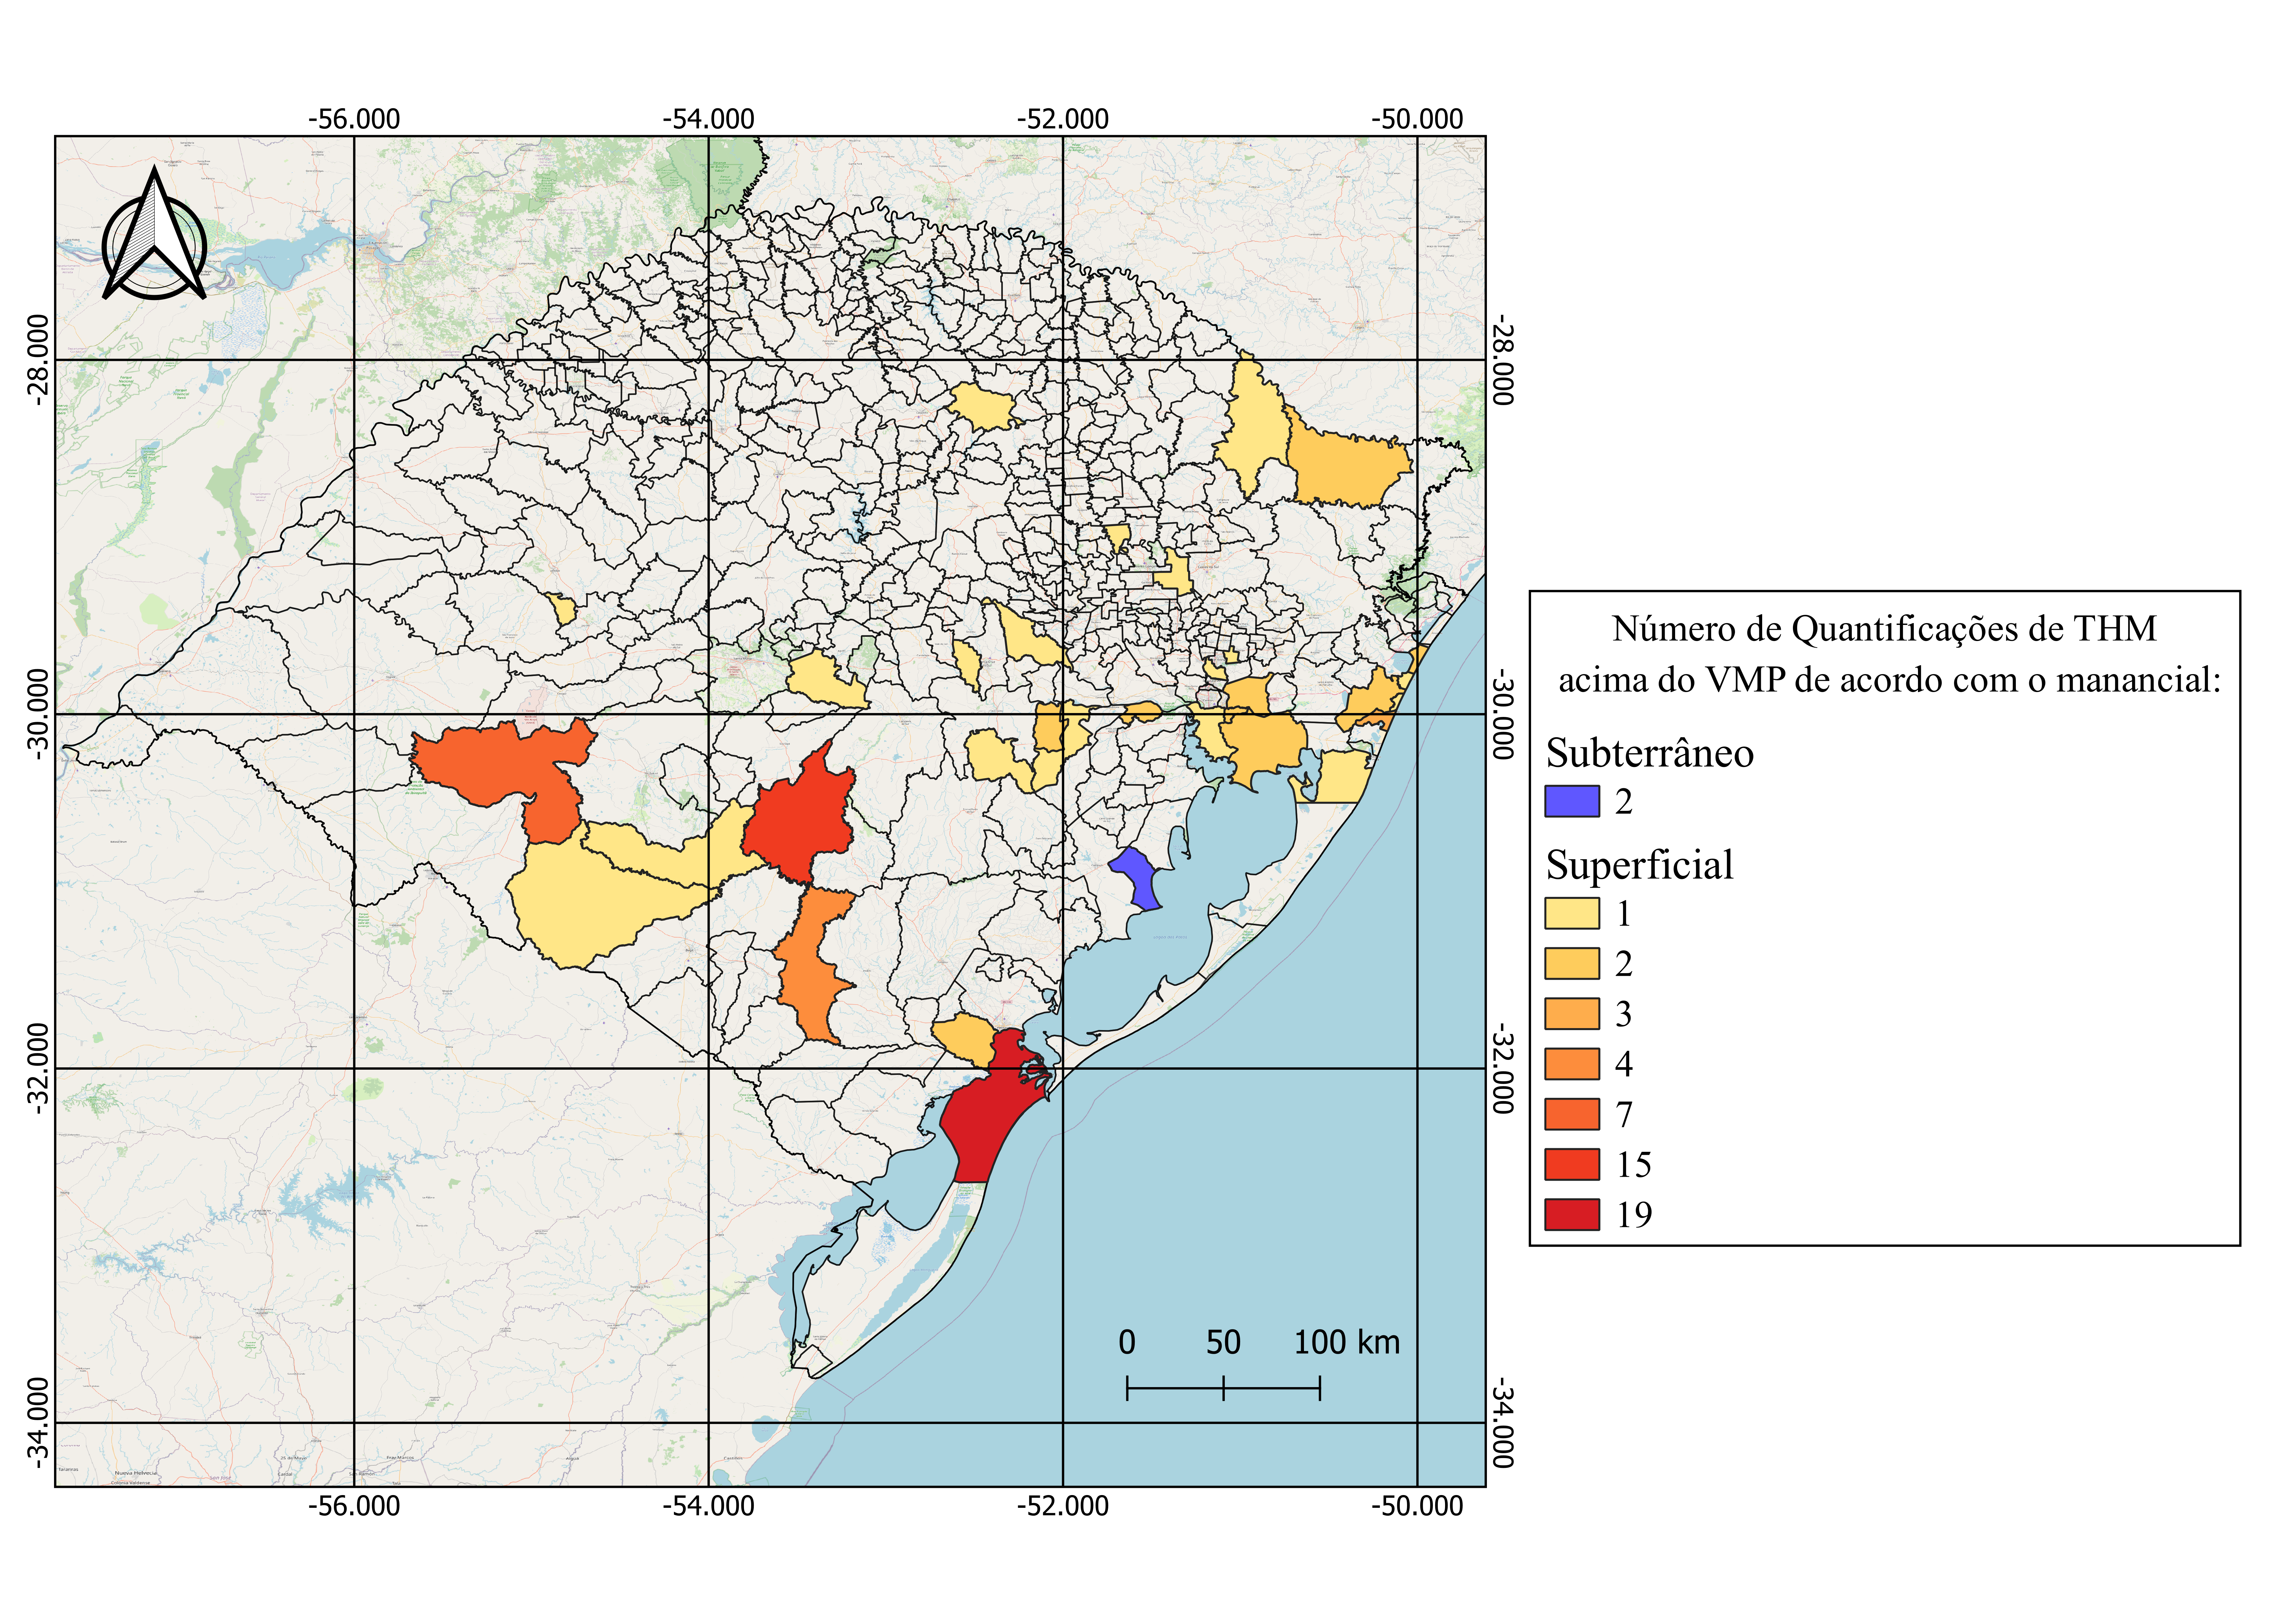
\includegraphics[scale=0.56]{images/cc.png}
\label{fig04}
\end{figure}


%A variação sazonal está relacionada ao aumento da temperatura do ar e às mudanças na quantidade e na qualidade da MON dos mananciais. Como os THMs podem ser formados durante as reações entre o cloro e a matéria orgânica, um nível mais alto de carbono orgânico dissolvido provavelmente formará mais THMs. 

\newpage

\section{Concentração dos quatro tipos de THMs no período de 2014 a 2015
}

A Tabela 13 apresenta os dados referente ao número de análises e de presença dos quatro componentes do THM separadamente entre 2014 e 2015, estes dados foram obtidos a partir dos relatórios da CORSAN antes da adequação dos relatórios no formato do Sisagua que considera somente trihalometanos totais. Foram analisadas 13.204 amostras com um percentual de formação de THMs de 26,5\%. A cinética de formação de THMs é inicialmente muito rápida e depois diminui \cite{mouly2010variations}, por esse fato, a máxima concentração encontrada foi na água tratada com concentração de 0,208 $mg.L^-^1$ e percentual de presença de THMs de 21,3\%. A análise proveniente da rede de distribuição obteve percentual de formação mais elevado que a água tratada, porém, com concentração máxima menor. Variações temporais na concentração de PSDs e cloro residual livre podem ser influenciadas pelo tempo de residência da água na rede \cite{mouly2010variations}.


\begin{table}[!htb]
\centering
\small
\caption{\small Número de análises e de presença dos quatro componentes dos trihalometanos  no Rio Grande do Sul entre 2014 e 2015.}
\label{tab:com_esp}
    \begin{tabular}{p{3.3cm}p{0.9cm}p{0.9cm}p{1cm}p{1cm}p{1.2cm}p{1.2cm}}
    \toprule
    \textbf{Matriz} & \textbf{N} & \textbf{NP}& \textbf {\%NP}&\textbf{Média} & \textbf{Mínimo} &\textbf{Máximo}\\ \hline
      Água Bruta   & 24 & 3 & 12,5\% & 0,004 & 0,0015 & 0,008 \\
      Água Tratada & 8470 & 1803 & 21,3\% & 0,009 & 0,0006 & 0,208\\
      Rede de Distribuição & 4710 & 1693 & 35,9\% & 0,011 & 0,0006 & 0,182\\ \hline
      \textbf{Total} & \textbf{13204} & \textbf{3499} & \textbf{26,5\%} & \textbf{0,01} & \textbf{0,0006} & \textbf{0,208} \\
      \bottomrule
    \end{tabular}
    \legend{\footnotesize N: número de análises; NP: número de presença;NP\%: percentual do número de presença; Média, Mínimo e Máximo: $mg.L^-^1$\\}
    \label{tab01}
\end{table}

\newpage
A Tabela 14 apresenta a ocorrência dos quatro componentes dos THMs em manancial de abastecimento e em águas tratadas no RS entre 2014 e 2015. 
Estudos anteriores confirmaram que alguns íons na água têm efeitos significativos na formação de PSDs. O íon mais extensivamente investigado é o $Br^-$ que está amplamente presente nas águas subterrâneas ou superficiais, especialmente em cidades costeiras devido à introdução de água salgada \cite{Nata2020}.  Em todos os mananciais há predominância do clorofórmio e bromodiclorometano e a maior concentração corresponde ao dibromoclorometano  (0,208 $mg.L^-^1$). Os valores condizem com a literatura, pois o clorofórmio é o THM mais comum em água clorada \cite{who2005}. No estudo de \cite{Abbas2014} a ocorrência de THMs foi encontrada na seguinte ordem: clorofórmio = bromodiclorometano > dibromoclorometano > bromofórmio, o que vai ao encontro dos dados da CORSAN de 2014 a 2015.

O íon $Br^-$ é o precursor iônico para a formação de THM bromados. Quanto maior a presença do íon na água bruta a ser tratada, maior será a substituição $Br^-$ em THM clorados para a formação de espécies mais bromadas \cite{Nata2020}. Por isso, a ocorrência de espécies bromadas, principalmente o bromofórmio, é baixa para todos os mananciais presentes na Tabela 11.



\begin{table}[!htb]
\begin{flushleft}
\small
\caption{\small Ocorrência dos quatro componentes dos trihalometanos por manancial de abastecimento no Rio Grande do Sul entre 2014 e 2015.} \label{tab:com_esp}
\centering
\begin{tabular}{p{2cm}p{3.2cm}p{1cm}p{0.6cm}p{1.2cm}p{1cm}p{1cm}p{1cm}}
\toprule
\textbf{Manancial}  & \textbf{Parâmetro}& \textbf{N} & \textbf{NP} & \textbf{NP\%} &  \textbf{Mín.}  & \textbf{Máx.} & \textbf{Média} 
 \\
\midrule
& Bromodiclorometano & 715 & 303 & 42,4\% & 0,0011 & 0,011 & 0,003\\
Superficial & Bromofórmio & 696 & 16 & 2,3\% & 0,0009 & 0,164 & 0,002\\
& Clorofórmio & 776 & 388 & 50\% & 0,0009 & 0,056 & 0,004\\
& Dibromoclorometano & 761 & 92 & 12,1\% & 0,0006 & 0,208 & 0,010\\\hline

& Bromodiclorometano & 585 & 222 & 37,9\% & 0,0006 & 0,046 & 0,004\\
Misto & Bromofórmio & 611 & 17 & 2,8\% & 0,001 & 0,013 & 0,004\\
& Clorofórmio & 601 & 307 & 51,8\% & 0,0009 & 0,154 & 0,016\\
& Dibromoclorometano & 608 & 67 & 11\% & 0,0009 & 0,039 & 0,004\\
\hline
& Bromodiclorometano & 2005 & 821 & 41\% & 0,0006 & 0,031 & 0,004\\
Subterrâneo & Bromofórmio & 1983 & 35 & 1,7\% & 0,001 & 0,032 & 0,004\\
& Clorofórmio & 1933 & 988 & 51,1\% & 0,0009 & 0,046 & 0,004\\
& Dibromoclorometano & 1930 & 243 & 12,6\% & 0,0006 & 0,026 & 0,004\\

\bottomrule
\end{tabular}
\legend{\footnotesize N: número de análises; NP: número de presença; NP\%: percentual do número de presença; Mín.: Concentração mínima ($m g.L^-^1$); Máx.: concentração máxima ($m g.L^-^1$);  Média: ($m g.L^-^1$)}
\end{flushleft}
\end{table}

\newpage
A Tabela 15 apresenta dados dos quatro componentes dos THMs por ponto de coleta no RS entre 2014 e 2015. Embora o predomínio de análises seja na água tratada, o percentual de amostras com  presença de THMs é na água da rede de distribuição para todos os compostos presentes nos THMs. Esse efeito pode ser explicado quando, ao longo da rede de distribuição ocorre a diminuição do cloro residual livre adicionado na estação de tratamento. Nessas situações, a adição de cloro livre na rede de distribuição (recloração) provoca o reinício da formação de THMs \cite{mouly2010variations}.



\begin{table}[!htb]
\begin{flushleft}
\small
\caption{\small Ocorrência dos quatro componentes dos trihalometanos por ponto de coleta no Rio Grande do Sul entre 2014 e 2015.} \label{tab:com_esp}
\centering
\begin{tabular}{p{3cm}p{3.3cm}p{1cm}p{0.6cm}p{1.2cm}p{1.1cm}p{1.1cm}p{1.1cm}}
\toprule
\textbf{Parâmetro}  & \textbf{Ponto de Coleta}& \textbf{N} & \textbf{NP} & \textbf{NP\%} &  \textbf{Mín.}  & \textbf{Máx.} & \textbf{Média} 
 \\
\midrule
& Água Bruta & 6 & 1 & 16,67\%& 0,00272 & 0,00272 & 0,00272\\
Bromodiclorometano & Água Tratada & 2117 & 689 & 32,55\% & 0,00055 & 0,0311 & 0,00312\\
& Rede de Distribuição & 1182 & 656 & 55,50\% &0,00055 & 0,046&0,00423\\
\hline
& Água Bruta & 6 & 0 & 0\% & 0 & 0 & 0 \\ 
Bromofórmio & Água Tratada & 2118 & 22 & 1,04\% & 0,00115 & 0,0094 & 0,00324\\
& Rede de Distribuição & 1166 & 46 & 3,95\% & 0,00097 & 0,0324 & 0,00421\\\hline
& Água Bruta & 6 & 1 & 16,67\% & 0,008 & 0,008 & 0,008\\ 
Clorofórmio & Água Tratada & 2117 & 1114 & 43,98\% & 0,00092 & 0,208 &0,01473\\
& Rede de Distribuição & 1187 & 751 & 63,27\% & 0,00092& 0,182 & 0,01952\\\hline
& Água Bruta & 6 & 1 & 16,67\% & 0,00149 & 0,00149 & 0,00149\\ 
Dibromoclorometano &Água Tratada & 2118 & 161 & 7,60\% & 0,00088 & 0,044 &0,00334\\
& Rede de Distribuição & 1175 & 240 & 20,43\% & 0,00089& 0,056 & 0,00428\\
\bottomrule
\end{tabular}
\legend{\footnotesize N: número de análises; NP: número de presença; NP\%: percentual do número de presença; Mín.: Concentração mínima ($mg.L^-$); Máx.: concentração máxima ($mg.L^-$);  Média: ($mg.L^-$).}
\end{flushleft}
\end{table}


A presença de íon brometo ($Br^-$) que é oxidado em ácido hipobromoso (HOBr) impacta a formação de THMs bromados, com maiores riscos à saúde do que seus análogos clorados \cite{uyak2007investigation}. Com isso, a Figura 8 mostra a faixa de concentração do número de análises com presença de THMs bromados no RS entre 2014 e 2015. A ocorrência prevalece em municípios litorâneos e as máximas concentrações predominam no litoral norte do RS, devido a introdução da água do mar. No entanto, são 240 municípios que apresentaram em algum momento a concentração de THM bromado entre 2014 e 2015 no Rio Grande do Sul.


\begin{figure}[!htb]
\caption{\small Faixa de concentração para os componentes do THM que possuem bromo na composição  no RS entre 2014 e 2015.}
\centering
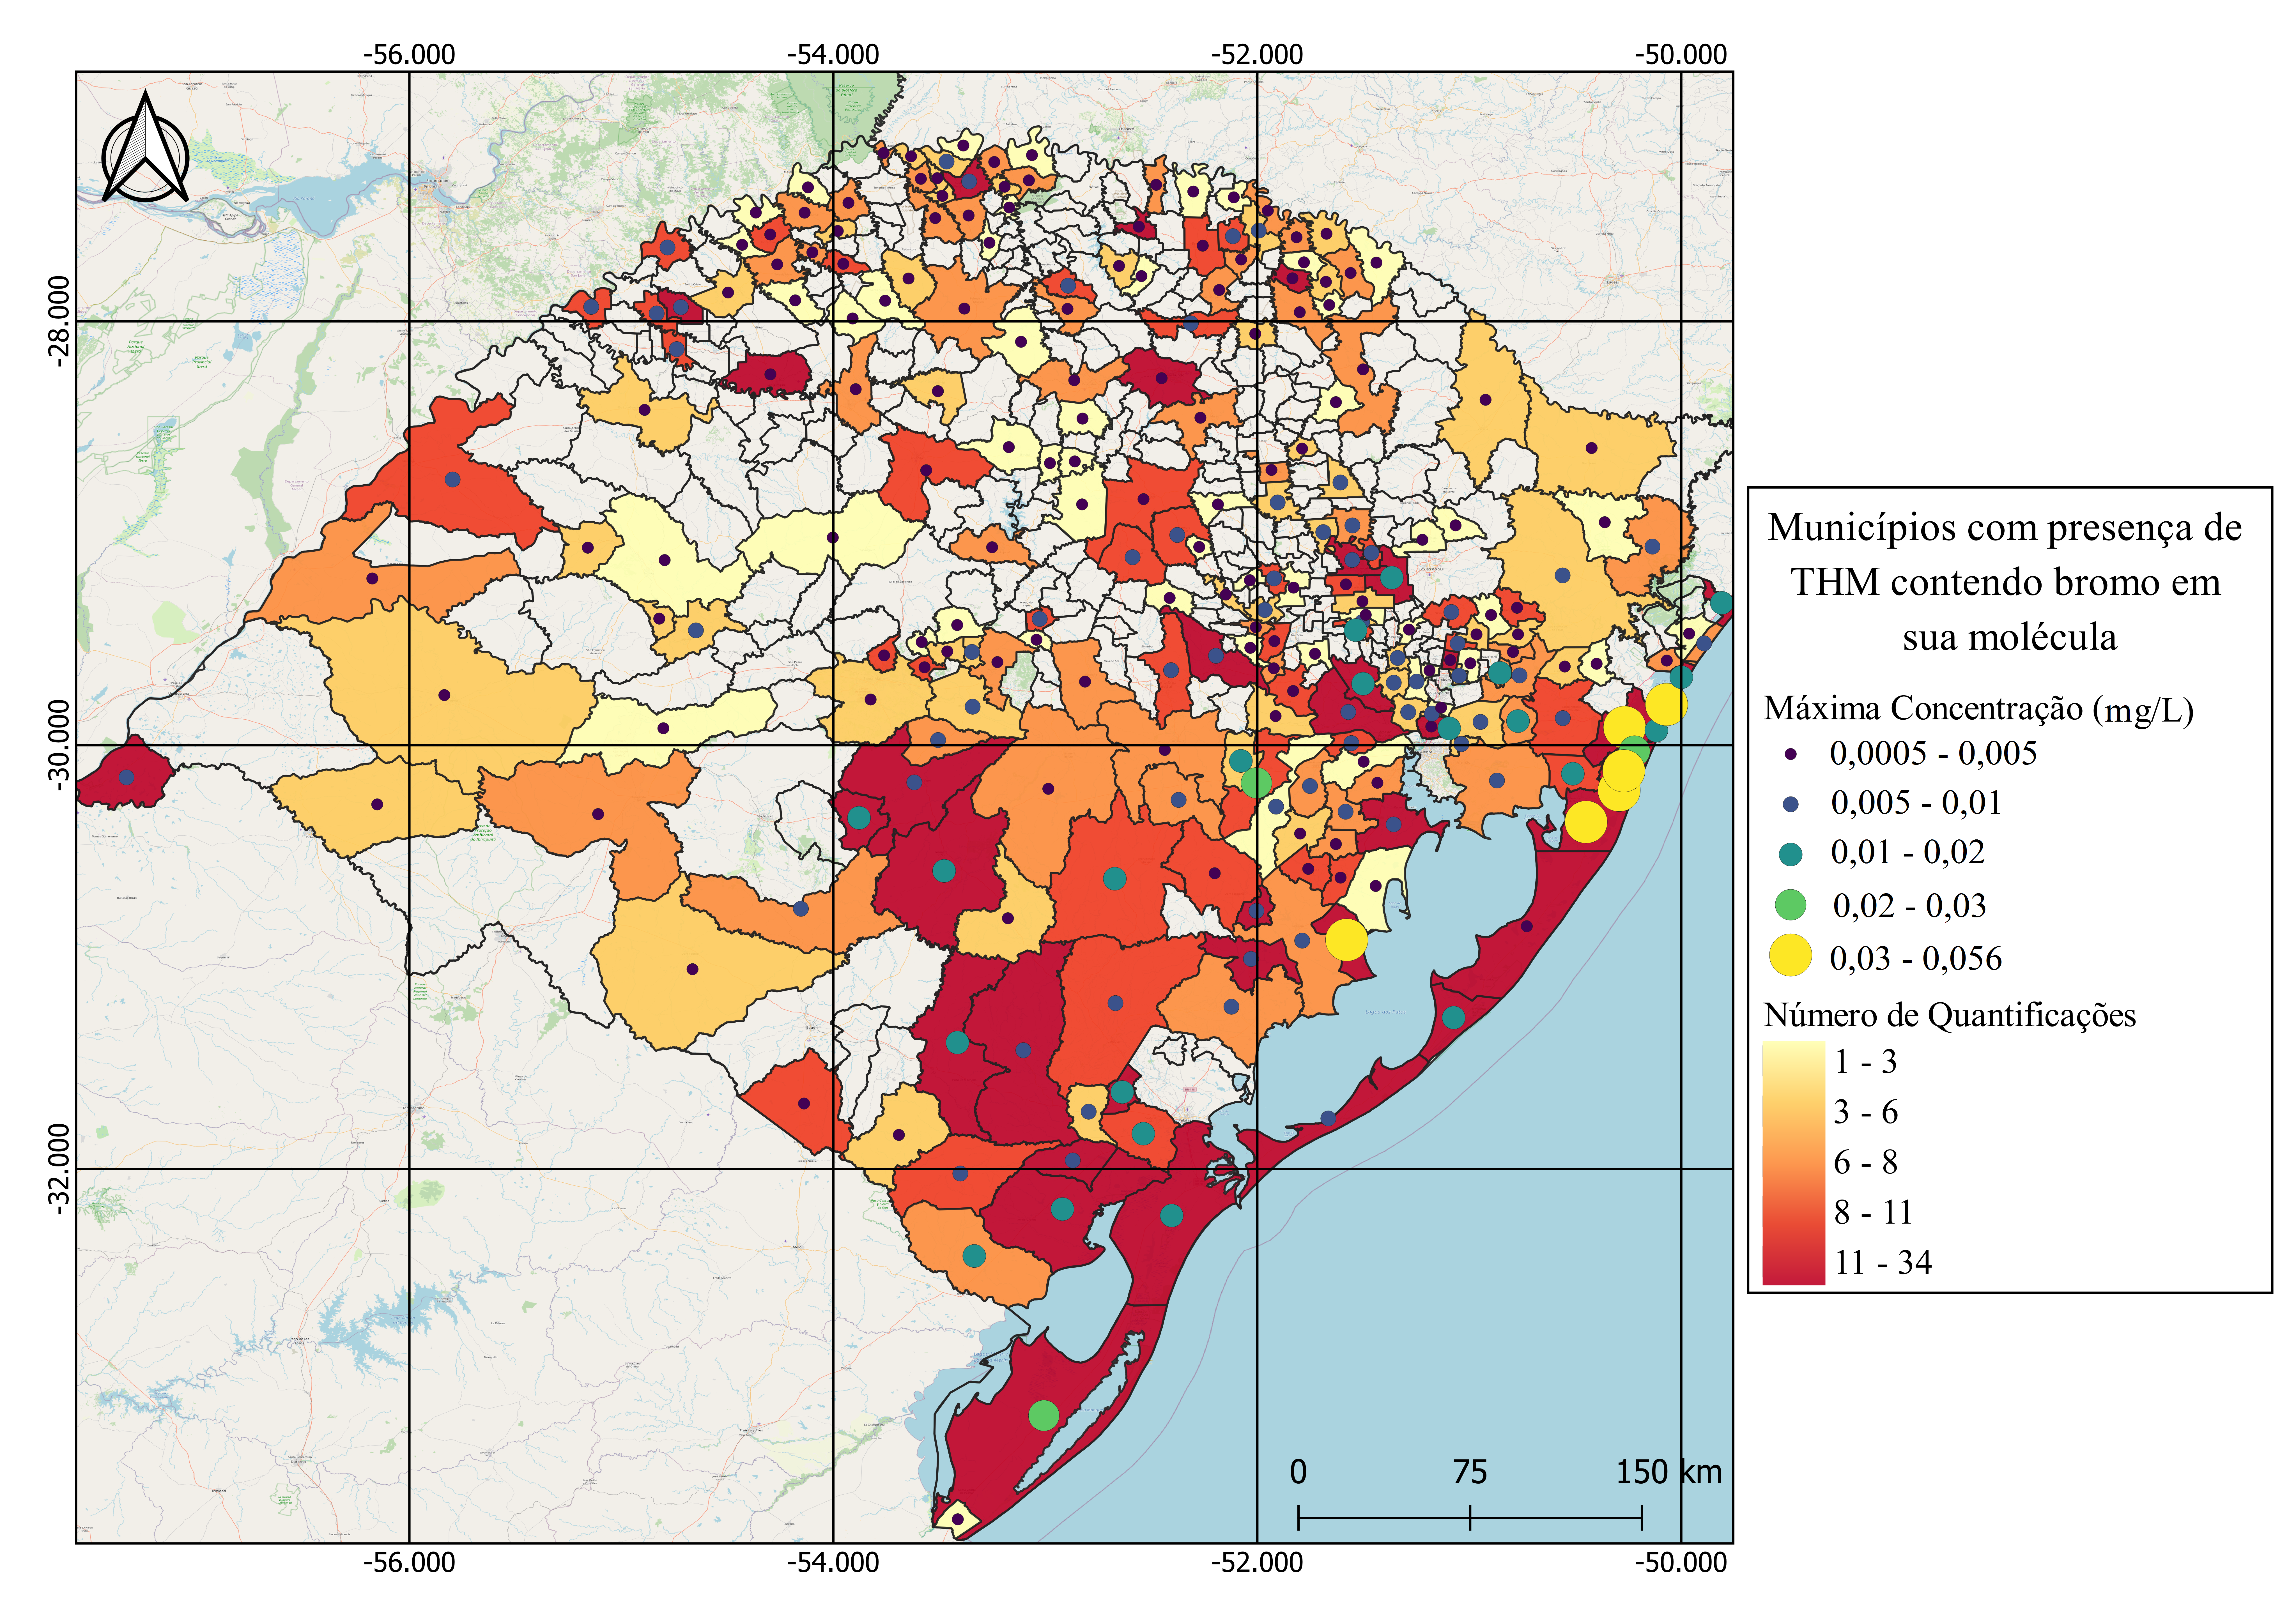
\includegraphics[scale=0.077]{images/bromo1.png}
\label{fig03}
\end{figure}


%%%%%%%%%%%%%%%%%%%%%%%%%%%%%%%%%%%%%%%%%%%%%%%%%%%%%%%%%%%%%%%%%%%%%%%%%5
%%%%%%%%%%%%%%%%%%%%%%%%%%%%%%%%%%%%%%%%%%%%%%%%%%%%%%%%%%%%%%%%%%%%%%











%Pesquisas anteriores mostraram que os fatores individuais que afetam mais fortemente a formação de THM são a dose de cloro e a concentração residual, tipo e quantidade de matéria orgânica, pH e temperatura da água e presença de brometo. \cite{SERRANO2015246}  nenhuma das espécies de THMs estudadas foi encontrada na água bruta em qualquer momento, com isso, concluiu que  a presença desses compostos na água tratada pode ser atribuída exclusivamente ao processo de desinfecção.





% SERRANO A concentração de TCM foi maior nos meses mais quentes (primavera e verão). As etapas de coagulação / floculação e sedimentação com policloreto de alumínio (SP3) ocasionaram a formação de outro THM (BDCM) e um HNM (TCNM) nas estações mais quentes,


%\cite{CUNHA2016516}
%O THMPF foi afetado pelo uso da terra e estação ( Tabela 5 ). Os maiores valores foram observados em áreas industriais / urbanas e agrícolas (média de 304  μg / L para ambos) quando comparadas às áreas florestais (231  μg / L) ( Fig. 2 ), refletindo um risco de formação de tais compostos ∼24% menor se a água bruta veio de rios ou córregos localizados em áreas com mais remanescentes nativos ou vegetação recuperada.



%Os valores de THMPF observados são relativamente altos e a pré-cloração deve ser evitada em todas as ETAs locais, independentemente do principal uso do solo na bacia. Métodos alternativos para cloração e sua eficiência para desinfecção estão disponíveis (por exemplo, Li et al., 2011 ).



% Conforme o conteúdo de cloro aumentou, a concentração de THMs também aumentou. No entanto, a formação máxima de THMs (ou THMFP) ocorreu na dose de cloro de 20  mg / L, ou seja , 217,5  µg / L. o THMFP na reação de 23  mg / L de cloro com a origem de NOM aumenta linearmente com o aumento da temperatura da água. Geralmente, uma elevação da temperatura acelera a taxa de reação e o conteúdo orgânico das águas [25] . Se os produtos são relativamente estáveis, suas formações aumentam com a temperatura. Conforme mostrado na Fig. 2 b, uma forte relação foi observada entre THMFP e temperatura da água. Na faixa de temperatura da água estudada (5–35  ° C), a variação no THMFP foi pequena na água fria (temperatura da água <15 ° C) em comparação com as temperaturas mais elevadas (temperatura da água> 15  ° C). 

%CFM e BDCM diminuíram continuamente; O DBCM aumentou inicialmente, mas depois diminuiu e sua concentração máxima ocorreu nas concentrações de brometo de 150  μg / L para as respectivas doses de cloro; O BFM aumentou continuamente, exceto para os níveis de 20  mg / L de cloro e 250  μg / L de Br - . Para ambas as concentrações de cloração, os rendimentos de THMs testados foram melhorados conforme o nível de brometo aumentou (Fig. 4 ). Isso ocorre porque o íon brometo pode ser oxidado pelo cloro livre para produzir ácido hipobromoso (HOBr). Semelhante ao ácido hipocloroso (HOCl), o HOBr reagiu com o NOM e exibiu uma capacidade de substituição muito mais poderosa do que o HOCl [29] , [30] . Estes resultados são consistentes com relatórios anteriores. O aumento das concentrações de cloro e dos níveis de brometo resultou em um aumento consistente dos níveis de THMs totais devido à produção de maior nível de HOBr.
%os níveis de THMFP foram especialmente altos no verão e baixos durante a primavera e o outono. De fato, os níveis médios medidos de THMs durante o verão na água bruta do Rio Dez foram 1,73 vezes maiores do que os da primavera. O conteúdo de salinidade (Br - e Cl - ) da água aumentou com o aumento da temperatura no verão. Concluiu-se que as variações sazonais nos PADs estão relacionadas às mudanças na quantidade e na qualidade do NOM dos mananciais. Como os THMs podem ser formados durante as reações entre o cloro e a matéria orgânica, um nível mais alto de carbono orgânico dissolvido provavelmente formará mais THMs. 




%\cite{LI2021116712}
%A concentração de clorofórmio mostrou ter uma relação negativa com as concentrações de dibromoclorometano e bromofórmio. Por exemplo, em sistemas com baixo teor de brometo (Sydney), observou-se que o clorofórmio é a espécie THM dominante com um nível insignificante de bromofórmio. Em contraste, as concentrações de Br-THMs foram observadas como abundantes no sudeste de Queensland. Como antecipado, bromodiclorometano e dibromoclorometano foram as espécies mais abundantes quando a concentração de clorofórmio era baixa. Espera-se que um fator importante na produção desse resultado sejam as concentrações mais altas de brometo na fonte de água do sudeste de Queensland, mas outras diferenças operacionais potenciais também podem desempenhar um papel. Isso inclui as concentrações de cloro livre e monocloramina que podem levar a proporções variáveis de Cl: Br. Este deslocamento de especiação é consistente com relatórios anteriores, indicando que a presença de brometo pode deslocar a especiação de Cl-THMs para Br-THMs.
%As principais conclusões deste estudo são:
%A monocloramina tem uma correlação negativa com a formação de THMs, indicando que a degradação gradual da monocloramina leva à formação conseqüente de THMs em DWDSs.

%A alta concentração de cloro livre está associada à alta formação de THMs, especialmente Cl-THMs, o que provavelmente reflete a redução do cloro livre dentro do sistema de distribuição após um declínio significativo da monocloramina.

%Gerenciar a degradação da monocloramina pode ser uma estratégia eficaz para controlar a formação de THM, que pode ser alcançada mantendo uma faixa de pH mais alta.

%Consistente com o entendimento atual, baixas concentrações de DOC e TDS levam à redução da formação de THM em DWDSs. Assim, a formação de THM pode ser gerenciada minimizando DOC e TDS nos DWDSs, especialmente durante as estações mais quentes.

%Aplicar pH mais alto é uma alternativa para reduzir a formação de THM quando baixas concentrações de TDS são difíceis de alcançar. No entanto, o pH alto está associado à baixa concentração de cloro livre, o que aumenta a probabilidade de maior formação de Br-THMs em água com alta concentração de brometo devido às menores razões Cl: Br.
%-Condutividade mais baixa e TDS estão associados com a minimização da formação de bromofórmio, indicando que eles são uma medida substituta razoável para íons de brometo.









%\cite{DU2021144662} No geral, a concentração de clorofórmio foi a maior para todos os métodos de desinfecção, com média de 13,3 μg / L. E a concentração de BDCM foi próxima ao clorofórmio. A concentração de bromofórmio foi a mais baixa entre os seis DBPs.
%No geral, as concentrações de DBPs na água potável na estação chuvosa foram maiores do que na estação seca. Havia mais DBPs na água potável urbana do que na rural. Os DBPs na água potável usando água subterrânea como matéria-prima eram mais do que usando água superficial.


% 

%\cite{Abbas2014} ao comparar duas cidades do Paquistão, Islamabad e Rawalpindi, a primeira abastecida por captação superficial e a segunda por captação subterrânea, os resultados mostraram maior concentração de TTHMs em Islamabad. Captação subterrânea possui menor concentração de MON. A água superficial foi suscetível a conter maior matéria orgânica em comparação com a água de poço devido ao excesso de vegetação e alta temperatura ao longo do ano. O tratamento com cloro dessas águas superficiais, com maior quantidade de matéria orgânica.Assim, o clorofórmio sozinho contribuiu com mais de 90\% em todos os locais de amostragem. O BDCM e o DBCM deram uma contribuição trivial de 5–10\% e 0–5\%, respectivamente. Bromofórmio apresentou uma contribuição quase insignificante.. O clorofórmio foi comparativamente menor em concentração em tanques subterrâneos.

%Geralmente, a desinfecção das águas superficiais produz mais THMs em comparação com as águas subterrâneas devido à presença de alta matéria orgânica ( Hassan et al. 2010 ).

%\cite{Nata2020} bromo.

%O potencial de formação de trihalometanos (PFTHM) é uma metodologia utilizada para avaliar a possibilidade de formação de subprodutos da desinfecção (SPD) por cloração durante o processo de tratamento da água. Em estudo desenvolvido a partir de PFTHM, encontrou-se para cada parâmetro que compõe os THMs, observou-se que 80,9\% dos THM formados consistiram no clorofórmio, 16,4\% representam o diclorobromometano e 2,7\%, o dibromoclorometano. O tempo de reação do cloro com a MON contribuiu diretamente para a formação de THM. Além disso encontrou correlação entre THM com a dureza, ou seja, a formação de THM é diretamente proporcional ao aumento da dureza da água. Os íons Ca2+ e Mg2+ podem contribuir para o aumento da formação de THM \cite{oliveira2020}.



%Os estudos anteriores confirmaram que alguns íons na água têm efeitos significativos na formação de DBP. O íon mais extensivamente investigado é o Br - que está amplamente presente nas águas subterrâneas ou superficiais, especialmente em cidades costeiras devido à intrusão de água salgada; a maior concentração de Br - sobe para vários miligramas / litro (Liu et al. 2011 ; Tian et al. 2013 ). Além disso, como um ingrediente variado de hipoclorito comerciais desinfectante de uso geral, Br - entra beber sistema de tratamento de água. Os estudos aprovaram por unanimidade que Br -é um precursor iônico significativo de Br-DBPs, contribuindo para a formação de Br-DBPs e TOBr desconhecido, e mais significativamente, Br - muda Cl-DBPs para espécies mais bromadas (Chang et al. 2001 ; Padhi et al. 2019 )

%[https://link.springer.com/article/10.1007/s11270-020-04786-6]

%https://www.sciencedirect.com/science/article/pii/S0045653517304769

%https://www.sciencedirect.com/science/article/pii/S0048969719303018


%\cite{cancer}


% ||||||||||||||||||||||||||||||||||||||||||||||
% CONCLUSÃO (capítulo sem numeração e presente no sumário)
% ||||||||||||||||||||||||||||||||||||||||||||||
%\chapter*[Conclusão]{Conclusão}
%\addcontentsline{toc}{chapter}{Conclusão}
% Utilize caso a conclusão seja um capitulo sem numeracao.

% ||||||||||||||||||||||||||||||||||||||||||||||
% CAPITULO 5
% ||||||||||||||||||||||||||||||||||||||||||||||
\chapter{Conclusão}

O presente estudo comparou a ocorrência, formação e risco à saúde de THMs em água para consumo humano.

As principais conclusões deste trabalho são, ressaltando que o § 5º do Art. 44 da Portaria MS Nº 888/2021 (antigo § 6º do Art. 41 no Anexo XX da Portaria de Consolidação Nº 5/2017): \textit{"Na verificação do atendimento ao padrão de potabilidade expressos nos Anexos 9 a 11, a detecção de eventuais ocorrências de resultados acima do VMP deve ser analisada em conjunto com o histórico do controle de qualidade da água."}:

\begin{itemize}
  \item Foram analisadas 17.245 amostras, o que representa aproximadamente 47\% do cumprimento do plano de amostragem previsto para análise do padrão de potabilidade de THMs;

  \item  1.925.192 pessoas foram expostas a concentração de THMs acima do VMP em 33 municípios em algum momento entre 2014 a 2020;
  
  \item 46 municípios descumpriram o padrão brasileiro de potabilidade pela ausência de análises de THMs;
  
  \item A água dos sistemas abastecidos por manancial superficial apresentou maior concentração de THMs comparada aos tipos de manancial, subterrâneo e misto;
  
  \item A presença de THMs em água bruta em 2016 e 2017 mostrou possível pré-cloração em água proveniente de manancial superficial com presença de precursores de formação de THMs (matéria orgânica);
  
  
  \item Água bruta de sistemas abastecidos por manancial subterrâneo com presença de THMs sugere a necessidade de processos de tratamento da água anteriores ao processo da desinfecção; 
  
  
  \item A correlação de Spearman  mostrou que o aumento de chuva ou temperatura ocasiona um aumento de concentração de THMs;
  
  \item A presença de concentrações de clorofórmio e bromodiclorometano foram maiores comparadas ao bromofórmio e dibromoclorometano no período de 2014 e 2015.
 
  \item Componentes do THM que possuem bromo na composição estão presentes em 240 municípios do RS, especialmente em cidades costeiras devido à introdução de água do mar;

  \item Como possíveis ações para reduzir a concentração de THMs pode-se otimizar a clarificação para remoção de precursores, reduzir a concentração de cloro ou substituir o produto de desinfecção.

\end{itemize}
 
\section{Trabalhos Futuros}


\begin{itemize}
 \item Correlacionar resultados de presença de THMs com dados de câncer de bexiga e colorretal no Estado do Rio Grande do Sul;
 
 \item Estimar a concentração de ácidos haloacéticos a partir da concentração de THMs no período de 2014 a 2015 pela metodologia de Roberts \textit{et al.} (2002) \cite{roberts2002}.

\end{itemize}

% ----------------------------------------------
% Finaliza a parte no bookmark do PDF para que se inicie o bookmark na raiz e adiciona espaço de parte no Sumário
% ----------------------------------------------
%\phantompart

% Arquivo de elementos pós-textuais: referências, apêndices e anexos 
% ==============================================
% ELEMENTOS PÓS-TEXTUAIS
% ==============================================
\postextual

% ||||||||||||||||||||||||||||||||||||||||||||||
% REFERÊNCIAS BIBLIOGRÁFICAS
% ||||||||||||||||||||||||||||||||||||||||||||||
\bibliography{references}

% ----------------------------------------------
% Glossário
% ----------------------------------------------
% Consulte o manual da classe abntex2 para orientações sobre o glossário.
%
%\glossary

% ||||||||||||||||||||||||||||||||||||||||||||||
% APÊNDICES
% ||||||||||||||||||||||||||||||||||||||||||||||
\begin{apendicesenv}

\partapendices

% ----------------------------------------------
% Apêndice 1
% ----------------------------------------------
\chapter{CÓDIGO NO PYTHON}

\begin{figure}[!htb]
\centering
\includegraphics[scale=0.4]{colab/laudos 1.png}
\label{fig04}
\end{figure}

\begin{figure}[!htb]
\centering
\includegraphics[scale=0.4]{colab/laudos 2.png}
\label{fig04}
\end{figure}

\begin{figure}[!htb]
\centering
\includegraphics[scale=0.4]{colab/laudos 3.png}
\label{fig04}
\end{figure}

\begin{figure}[!htb]
\centering
\includegraphics[scale=0.4]{colab/laudos 4.png}
\label{fig04}
\end{figure}

% ----------------------------------------------
% Apêndice 2
% ----------------------------------------------
\chapter{Municípios que Não Possuem Resultados de THMs}

\begin{table}[!htb]
\centering
\footnotesize
\label{tab:com_esp}
    \begin{tabular}{lcc}
    \toprule
    \textbf{Município} & \textbf{Manancial} & \textbf{População Abastecida} \\ \hline
      Alto Feliz              & Subterrâneo        & 2.910                         \\
Anta Gorda              & Subterrâneo        & 4.188                         \\
Arroio do Padre         & Subterrâneo        & 1.386                         \\
Bom Princípio           & Subterrâneo        & 8.048                         \\
Candiota                & Superficial        & 7.843                         \\
Canudos do Vale         & Subterrâneo        & 485                           \\
Capão do Cipó           & Subterrâneo        & 1.444                         \\
Capitão                 & Subterrâneo        & 2.729                         \\
Cerro Branco            & Subterrâneo        & 764                           \\
Dois Lajeados           & Subterrâneo        & 1.683                         \\
Estrela Velha           & Subterrâneo        & 1.314                         \\
Forquetinha             & Subterrâneo        & 1.896                         \\
Gramado Xavier          & Subterrâneo        & 1.959                         \\
Guabiju                 & Subterrâneo        & 1.060                         \\
Herveiras               & Subterrâneo        & 1.968                         \\
Hulha Negra             & Subterrâneo        & 3.317                         \\
Ibarama                 & Subterrâneo        & 1.576                         \\
Imigrante               & Subterrâneo        & 1.984                         \\
Inhacorá                & Subterrâneo        & 1.449                         \\
Itacurubi               & Subterrâneo        & 1.358                         \\
Ivoti                   & Subterrâneo        & 20.720                        \\
Jari                    & Subterrâneo        & 1.047                         \\
Monte Alegre dos Campos & Subterrâneo        & 1.396                         \\
Muçum                   & Subterrâneo        & 4.862                         \\
Nova Pádua              & Subterrâneo        & 1.306                         \\
Novo Cabrais            & Subterrâneo        & 937                           \\
Paraíso do Sul          & Superficial        & 3.850                         \\
Passo do Sobrado        & Subterrâneo        & 5.109                         \\
Picada Café             & Subterrâneo        & 5.625                         \\
Pinhal da Serra         & Subterrâneo        & 432                           \\
Pinhal Grande           & Subterrâneo        & 774                           \\
Progresso               & Subterrâneo        & 3.060                         \\
Protásio Alves          & Subterrâneo        & 628                           \\
Quevedos                & Subterrâneo        & 1.640                         \\
Relvado                 & Subterrâneo        & 1.663                         \\
São Martinho da Serra   & Subterrâneo        & 2.129                         \\
São Valentim do Sul     & Subterrâneo        & 2.080                         \\
São Vendelino           & Subterrâneo        & 2.243                         \\
Segredo                 & Subterrâneo        & 2.827                         \\
Sério                   & Subterrâneo        & 891                           \\
Sinimbu                 & Subterrâneo        & 5.681                         \\
Toropi                  & Subterrâneo        & 945                           \\
Turuçu                  & Superficial        & 3.113                         \\
Vale Real               & Subterrâneo        & 5.698                         \\
Vespasiano Corea        & Subterrâneo        & 727                           \\
Westfalia               & Subterrâneo        & 3.007                         \\\hline
\multicolumn{2}{c}{\textbf{Total}}           & \textbf{131.751}              \\ \bottomrule
    \end{tabular}
    
    \label{tab01}
\end{table}




\end{apendicesenv}

% ||||||||||||||||||||||||||||||||||||||||||||||
% ANEXOS
% ||||||||||||||||||||||||||||||||||||||||||||||
%\begin{anexosenv}
% Imprime uma página indicando o início dos anexos
%\partanexos

% ----------------------------------------------
% Anexo 1
% ----------------------------------------------
%\chapter{Datasheet}\label{anexo1}
%\includepdf[pages=-]{pdfs/Datasheet.pdf}

% ----------------------------------------------
% Anexo 2
% ----------------------------------------------
%\chapter{Anexo 2}

%\end{anexosenv}

% ==============================================
% INDICE REMISSIVO
% ==============================================
\phantompart
\printindex
% ----------------------------------------------




% ----------------------------------------------
\end{document}
% ----------------------------------------------

% ||||||||||||||||||||||||||||||||||||||||||||||
% ALGUNS EXEMPLOS DE CODIGO LATEX
% ||||||||||||||||||||||||||||||||||||||||||||||

% ----------------------------------------------
%	Figure example
% ----------------------------------------------
% \begin{figure}[htp]
% \centering
% \caption{\label{fig:x} Aqui vai o caption da imagem.}
% \includegraphics[width = 0.9\linewidth ]{images/x.png}
% \legend{Fonte: Adaptado de \citeonline{x}.}
% \end{figure}

% ----------------------------------------------
%	Figure example
% ----------------------------------------------
%\begin{figure}[htp]
%\centering
%\includegraphics[width = 0.5\linewidth ]{dlayer.jpg}
%\caption{\label{fig:1}Complanar waveguide parameters using two dielectric layers \cite{cwccs}.} 
%\end{figure}

% ----------------------------------------------
%	Equation example \ref{eqn:1}
% ----------------------------------------------
%\begin{eqnarray}
%\epsilon _{r} & = & \epsilon _{r}'(1-i\tan(\delta))
%\label{eqn:1}
%\end{eqnarray}

% ----------------------------------------------
%	Complex equations example \ref{eqn:2}
% ----------------------------------------------
%\begin{eqnarray}
%C_{1} & = & 2\epsilon _{0}(\epsilon _{r1}-1)\frac{K(k_{1})}{K(k_{1}')}\nonumber\\
%& = & 2\epsilon _{0}(\epsilon _{r1}'-i\tan(\delta)\epsilon _{r1}'-1)\frac{K(k_{1})}{K(k_{1}')}\nonumber\\
%& = & 2\epsilon _{0}(\epsilon _{r1}'-1)\frac{K(k_{1})}{K(k_{1}')}-i2\epsilon _{0}(\tan(\delta)\epsilon _{r1}')\frac{K(k_{1})}{K(k_{1}')}\\
%C_{2} & = & 2\epsilon _{0}(\epsilon _{r2}-\epsilon _{r1})\frac{K(k_{2})}{K(k_{2}')}\nonumber\\
%& = & 2\epsilon _{0}(\epsilon _{r2}'-i\tan(\delta)\epsilon _{r2}'-\epsilon _{r1}'+i\tan(\delta)\epsilon _{r1}')\frac{K(k_{2})}{K(k_{2}')}\nonumber\\
%& = & 2\epsilon _{0}(\epsilon _{r2}'-\epsilon _{r1}')\frac{K(k_{2})}{K(k_{2}')}-i2\epsilon _{0}(\tan(\delta)\epsilon _{r2}'-\tan(\delta)\epsilon _{r1}')\frac{K(k_{2})}{K(k_{2}')}\\
%C_{vac} & = & 4\epsilon _{0}\frac{K(k_{0})}{K(k_{0}')}
%\label{eqn:2}
%\end{eqnarray}

% ----------------------------------------------
%	Table example \ref{tab:1} 
% ----------------------------------------------
%\begin{table}[htb]
%\caption{Constants and Parameters.}
%\begin{center}
%\begin{tabular}{|c|c|c|c|}
%\hline
%\bfseries CONSTANT & \bfseries VALUE & \bfseries CONSTANT & \bfseries VALUE \\
%\hline \hline
%$\epsilon _{0}$ & 8.8540$\times$10$^{-12}$ & $c$ & 299792458~m/s \\
%\hline
%$\epsilon _{r1}$ & 11.7 & $h_{1}$ & 300~$\mu$m \\
%\hline
%$\epsilon _{r2}$ & 7.5 & $h_{2}$ & 200~nm \\
%\hline
%$\delta _{1}$ & 10$^{-4}$ & $\delta _{2}$ & 10$^{-2}$ $\sim$ 10$^{-3}$ \\
%\hline
%\end{tabular}
%\end{center}
%\label{tab:1}
%\end{table}

% ----------------------------------------------
%	Complex table example \ref{tab:2}
% ----------------------------------------------
%\begin{table}[htb]
%\caption{Results and dimensions.}
%\begin{center}
%\begin{tabular}{|c|c|c|c|c|}
%\hline
%\bfseries $f_{0}$ [MHz] & \bfseries $S$ [$\mu$m] & \bfseries $W$ [$\mu$m] & \bfseries $d$ [cm] & \bfseries $C_{c}$ [fF] \\
%\hline
%\hline
%\multirow{4}{*}{650} & \multirow { 2}{*}{2} & \multirow{ 2}{*}{1} & \multirow{ 2}{*}{9.4966} & 10 \\
%\cline{5-5}
%& & & & 30 \\
%\cline{2-4} \cline{5-5}
%& \multirow { 2}{*}{4.5} & \multirow { 2}{*}{2.3} & \multirow { 2}{*}{9.3155} &         10 \\
%\cline{5-5}
%& & & & 30 \\
%\hline
%\multirow { 4}{*}{6000} &  \multirow { 2}{*}{2} &  \multirow { 2}{*}{1} &  \multirow { 2}{*}{1.0288} &          1 \\
%\cline{5-5}
%& & & & 3 \\
%\cline{2-4} \cline{5-5}
%& \multirow { 2}{*}{4.5} &  \multirow { 2}{*}{2.3} &  \multirow { 2}{*}{1.0092} &          1 \\
%\cline{5-5}
%& & & & 3 \\
%\hline

%\end{tabular}
%\end{center}
%\label{tab:2}
%\end{table}

% ----------------------------------------------
%	Two graphics in one \ref{fig:2}
% ----------------------------------------------
%\begin{figure}[htp]
%\centering
%\begin{tabular}{cc}
%(a) & (b) \\
%\includegraphics[width = 0.5\linewidth ]{DM_6G_4p5_3_6.jpg} &
%\includegraphics[width = 0.5\linewidth ]{DM_650_4p5_10_6.jpg}
%\end{tabular}
%\caption{captions} 
%\label{fig:2}
%\end{figure}

% ----------------------------------------------
%	Four graphics in one table \ref{fig:3}
% ----------------------------------------------
%\begin{figure}[htp]
%\centering
%\begin{tabular}{cc}
%(a) & (b) \\
%\includegraphics[width = 0.5\linewidth ]{DM_650_4p5_10_1.jpg} &
%\includegraphics[width = 0.5\linewidth ]{DM_650_4p5_30_1.jpg} \\
%(c) & (d) \\
%\includegraphics[width = 0.5\linewidth ]{DM_6G_4p5_1_1A.jpg} &
%\includegraphics[width = 0.5\linewidth ]{DM_6G_4p5_3_1.jpg} \\
%\end{tabular}
%\caption{Captions} 
%\label{fig:3}
%\end{figure}

% ----------------------------------------------
%	Quote and footnote
% ----------------------------------------------
%\begin{quote} ``adkfjahsldkfjashflkasdjfhadslkfjhasdlfkjadshflsda
%kjdshflkasjdfhalskfjhadslfksdajhfladskjfhsda
%kajsdfhlaksdjfhasdkl'' \footnote{test footnote}
%\end{quote}

% ----------------------------------------------
%	PDF Annotation
% ----------------------------------------------
%\pdfannot % generic annotation
%width 10cm % the dimension of the annotation can be controlled
%height 0cm % via <rule spec>; if some of dimensions in
%depth 4cm % <rule spec> is not given, the corresponding
% value of the parent box will be used.
%{ %
%/Subtype /Text % text annotation
%/Open true % if given then the text annotation will be opened
%/Contents % text contents
%(write comments in here...)
%}%
%

% ----------------------------------------------
% Tutorial para compilação offline
% ----------------------------------------------
% Faça o download dos seguintes softwares: Miktex (basic) e texStudio
% https://miktex.org/download
% http://www.texstudio.org/
% Instale o Miktex e selecione para instalar os pacotes automaticamente... Install Packages on the Fly = Yes
% Depois de instalado abra o "Miktex Package Manager (Admin)" e já instale os pacotes "abntex2" e o "cm-super".
% Instale o texstudio
% Faça o download dos arquivos do projeto no Overleaf "Download as ZIP"
% Descompacte no diretório de projeto desejado... use um diretório para cada projeto pois durante a compilação serão gerados diversos arquivos
% Abra o "main.tex" do projeto no texstudio e clique no icone >> para compilar o projeto... tecla de atalho = F5.


%%% -*-LaTeX-*-
%%% demo-tables.tex -- exemplo de tabelas.
%%% $Id: demo-tables.tex,v 1.9 2001/01/12 02:28:44 jessen Exp $

\section{Tabelas}
\index{tabelas|(}%

%%% l == column left-aligned
%%% r == column right-aligned
%%% c == column centered
%%% | vertical line
%%% || double vertical line

%%%%%%%%%%%%%%%%%%%%%%%%%%%%%%%%%%%%%%%%%%%%%%%%%%%%%%%%%%%%

